%!TEX root = ../dissertation.tex

\chapter{Background}
\label{chapter:background}
%
In this work, we introduce a review through the topics related to this project. We start by introducing
an explanatory view about Color Perception, narrowing it down to Color Philosophy and the Human Eye. Later,
we are going to introduce the theory behind Color Spaces and Models, ending this section with an overview about
the usage of Color Blending and the investigation that has been done, to understand the perception on this. In
the end, we will discuss the results found from this investigation was draft research questions which remain
unanswered.
%
\section{Theoretical Background}
\label{sec:theory_background}
%
This section contains the research performed to ascertain the theoretical background which supports our investigation.
We will begin by analizing the concepts \ul{Color Perception}, then briefly explaining the differences between \ul{Color
Models and Color Spaces}.
%
\subsection{Color Perception}
\label{subsec:colorperception}
%
In this section, we overview the philosophy about color, relating real-world perceptions to human perception
through the eye. There are two main areas of interest, called the Cones and the Rods, which will be explained
with quite detail; these areas restrict how we perceive color, specially if there are visual deficiencies.
Moreover, color creates mental models and codes, which are part of routines and rules followed by society, and will be exemplified in the end of this section.
%
\subsubsection{Color Philosophy}
\label{sec:colorphilosophy}
Looking up for a concrete definition of color is a hard task: there are quite a few ways to perceive color. Color
raises serious metaphysical questions\footnote{"Stanford Encyclopedia (...)", Available at: \url{www.stanford.io/1MWp7Zh}. Last accessed on October 17th, 2016.},
concerning the physical and psychological reality of it. Color is an
important feature of subjects: it allows us to recognize objects, locate them, it fires emotions and
behaviors and supports protocols over the world. Probably, the major problem of color has to do with what
we seem to know about it, into what physical properties of objects and materials express about them; David
Hume defended in 1739 \cite{Hume1739} that “(…) Sounds, colors, heat and cold, according to modern philosophy are not
qualities in objects, but perceptions in the mind (…)”, a highly subscribed dogma. This affirmation describes
two important tendencies, the \textbf{elimininativism} and the \textbf{subjectivism}: the first one is the
view that tells physical objects don’t have an inherent color associated to themselves, the last one states
that color is a subjective attribute of objects. Chirimuuta recently argued \cite{Chirimuuta2014} about the different
mindsets one can have regarding color: its main argument is that color is a subjective interpretation of
an objective physical stimuli and, to justify this statement, he settles a contrast between rival theories
of color. Color \textbf{realists} accept that colors are indeed physical properties of objects but instantaneously,
two questions arise from this: \textbf{1)} what really is color and its properties, and \textbf{2)} do objects really possess
those characteristics? With respect to these, we can derive more theories: \textbf{Primitivism}, \textbf{Reductive Physicalism},
\textbf{Dispositionalism}, among others. \par
%
Chirimuuta \cite{Chirimuuta2014} also compares the \textbf{Realism} against the \textbf{Anti-Realism}, since in the last one, the metaphysical question
“Can we say that objects are actually colored?” is promptly denied: colors do not physically and mentally
exist and nothing is, in fact, colored; it is even said by the anti-realists that classifying color by its features is an  illusion. As the author afirms, his view is close to \textbf{Relationism}, a theory which fills the gap
between the previous mindsets: to fathom color, we have to consider both the perception and the external
\emph{stimuli}, and treat color as the result of this interaction; the task of interpreting color is part of
the mechanism of accessing multiple properties of objects, as shape, composition, \emph{etc}.
Colors are, therefore, relational properties, with respect to perceivers and circumstances of viewing. \par
Regardless of which opinion you support, color has come to be an undeniable point of major interest of studies:
from philosophy, to psychology, computer science or statical analysis, color plays a major role in presenting
numbers, conveying ideas and spreading information. To endorse this usefulness, different color theories were
discovered all along the years and were accompanied by a profound research about the Human eye.
%
\subsection{The Human Eye}
\label{sec:humaneye}
%
The Animal visual system is a direct consequence of evolutionism: it is perfectly adjusted and adapted
to the way of living of every animal. We don’t hunt like wild animals, but our visual system is
prepared to distinguish a wide range of green colors since we evolved as a species surrounded by green
vegetation and knowing what to eat was a matter of life or death. The human visual system is adapted
to do many things, specially detecting sharpness and color with great precision and sensitivity during
the day light and night, although our night vision isn’t quite accurate. \par
%
Light is electromagnetic radiation, but most of this radiation is invisible to the human eye: it can
perceive light from under 400 nanometers until 750 nanometers.
When the light strikes an object, depending of the surface’s material, it can either: be wholly or partly
absorbed, reflected or transmitted; what we perceive as being an object is the light reflected of the
surface. The human eye, then, decodes light energy into neural activity:
this light reaches the eye through the \textbf{cornea}, crosses the pupil and is refracted by the lens, coming to a final
projection of a sharp image in the back of the eye, the \textbf{retina}. However, this image is
inverted, as the light rays from the top of the object are being project on the bottom of the retina,
so as the light rays coming from the right side of the object, projected in the left side of the
retina. This image is going to be rearranged by the brain.  \par
%
In order to be rearranged, the light is converted in the retina, which contains specialized cells
- photoreceptors - that convert light energy into neural impulses,
which are send to the brain. There are two main types of photoreceptors: \textbf{cones} and
\textbf{rods},
retinal cells that respond to light due to the absorption of photons in their proteins; cones are concentrated in the \textbf{fovea}. \par
%
The image is only sent to the brain after the signal generated by the cones and rods is processed also
in the bipolar cells of the retina, where visual information begins to be analyzed. After all, the brain digests the signals sent as we discussed
previously; moreover, as Attneave \cite{Attneave1954} states in its investigation in 1954, a major function of
the human perception mechanism is to strip way some redundant information present in the \emph{stimuli},
in order to encode or describe the incoming information in a more economical form, than the one in which
it impinges on the receptors. Likewise, sensorial events from different sensory systems may create
interdependencies among each other, either in space or in time, or crosscut both; over his life, any
individual acquires notions about “what-goes-with what” and, as the author states \cite{Attneave1954}, we cannot make
predictions about anything, based merely on the present visual field, but also depend on previous - and,
for that, familiar - visual fields. \par
As covered before, there are some specialized and important neurons
that have the crucial task of capturing and transducing photons: they convert electromagnetic radiation
into trigger-signals to be send to the organism.
The photoreceptors can be classified between \textbf{Cones} and \textbf{Rods}. \par
%
\paragraph{Cones}
%
\begin{wrapfigure}[10]{r}{0.3\textwidth}
	\centering
  \vspace{-\baselineskip}
	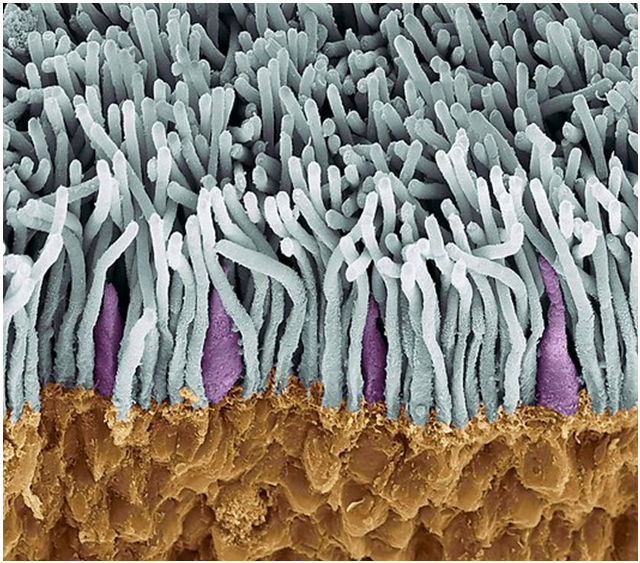
\includegraphics[width=0.3\textwidth]{images/background/Eye_ConesRods.png}
  \caption[Cones and Rods]{Cones and Rods.\protect\footnotemark{}}
  \label{fig:conesrods}
\end{wrapfigure}
\footnotetext{"The Human Eye and Adaptive Optics", Available at: \url{www.bit.ly/1zMEgK6}. Last accessed on October 17th, 2016.}
%
These cells are responsible for acquiring color vision information, at normal-to-high levels of bright
light. They are condensed in the fovea, which is a rod-free zone. By the time of 1990, in a study performed
by Curcio \emph{et al.} \cite{Curcio1990} it was estimated that in the human retina, the total number of cones ranged
between \ul{4.08 to 5.29 million}, Cone cells are not important to light detection, since they are not light
sensitive; however, color perception is completely instrumented by them. They can be seen on Figure \ref{fig:conesrods} as
being the pink colored structures.
These cells are named for their shapes and contain chemicals - the \emph{photospins} - that respond to light: when the
light strikes these chemicals, they break and create a signal which will be transferred to the brain.
There are three kinds of light-sensitive chemicals in cones and they will be providers for the basis
of color vision, creating the distinction between the number of cone types.
%
\begin{itemize}
	\setlength\itemsep{0.01em}
	\item \ul{S-Cones} (Small Wavelength Sensitive), correspond to Blue color perception.
	\item \ul{M-Cones} (Medium Wavelength Sensitive), correspond to Green color perception.
	\item \ul{L-Cones} (Large Wavelength Sensitive), correspond to Green-Red color perception.
\end{itemize} \par
%
The difference between the signals derived from the three types of cones, allows the brain to perceive a
continuous range of colors. The distribution of the amount of each type can differ.
%
\paragraph{Rods}
%
These photoreceptor cells function in less intense light, when compared to cone cells. They also acquire
their name because of their elongated, cylindrical shape (the white colored shapes in Figure \ref{fig:conesrods});
their location is on the outer edges of the retina, and the number of rods is around \ul{78 to 107 million}. These
cells are much more sensitive than
cones and they are responsible for night vision: in the dark, as your rods have only one type of light-sensitive chemicals (this is why your ability to see gradually increases in the dark). This limitation in the types of rods is the
reason why they cannot discriminate colors, as the cones. On Figure \ref{fig:colorsensitivity}, it is possible to compare
the light absorbance for different wavelenghts, distributed among Cones and Rods. \\ \par
%
\begin{figure}[H]
	\centering
    \vspace{-15pt}
    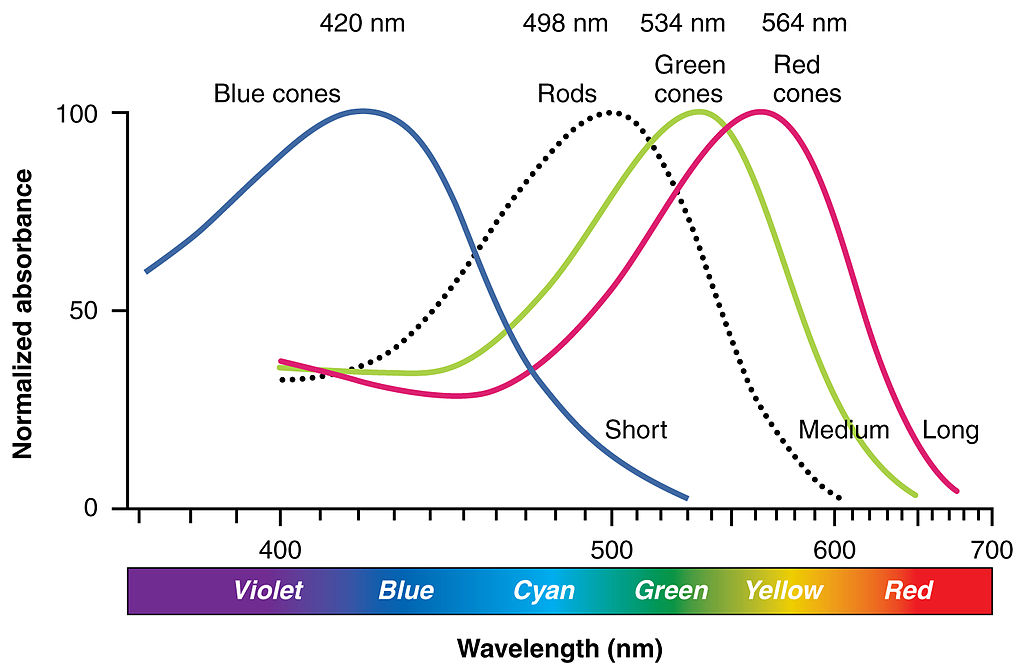
\includegraphics[width=0.5\textwidth]{images/background/Eye_Color_Sensitivity.jpg}
    \caption[Diagram of Eye Color Sensitivity]{Diagram of Eye Color Sensitivity, depicting distribution between cones and rods.\protect\footnotemark{}}
    \vspace{-15pt}
    \label{fig:colorsensitivity}
\end{figure}
\footnotetext{"Photoreceptor Cell", Available at: \url{www.bit.ly/1VNZQHE}. Last accessed on October 17th, 2016.}
%
All of this color information is, then, sent to the brain where it will be processed and associated to a
mental model. Psychologists tried to explain how the complete color vision works, and formulated some
theories about that.
%
\subsubsection{Theories of Color Vision}
The english physician Thomas Young published a theory \cite{Young1802}, where he stated that
in the human eye existed three types of photoreceptors, the cone cells. Later in that century, he was
joined by Hermann von Helmholtz when he concluded there exists three types of cone receptors and they could
be classified as short-preferring, middle-preferring and long-preferring, according to their response to
light’s wavelength. Together, they formed the \emph{Young-Helmholtz Theory}, or the so called \textbf{Trichromatic Theory}.
No single cone can detect by itself the color of a source of light: it is the ratio of the three types of cones that
determine what color will be sensed by the brain. This theory was largely applied in the creation of color
screens, for example televisions which contain microscopic elements of Red, Green and Blue. \par
\emph{Per contra}, german physiologist Ewald Hering developed in 1878 a theory: the
\textbf{Opponent Process Theory}. This theory suggest that our color perception is controlled by three
opponent pairs: red and green, blue and yellow, white and black\footnote{"How to See Impossible Colors (...)", Available at: \url{www.bit.ly/1ZdtSKv}. Last accessed on October 17th, 2016.}. Hering postulated that the members of each
pair either oppose or inhibit each other, only one element can be signaled at one time, but not both at the
same time: when one member of an opponent pair is no longer stimulated, the opponent pair is activated. For
example, if you stare for a long period of time to a red subject, when you look away the afterimage will be
red. \par
Together, these theories summarize what we know about color vision. The Trichromatic Theory explains how we see
what we see in color, but it is only valid for the presence of all types of cells. However, it has to be considered
the case in which these cells are totally or partially absent.
%
\subsubsection{Visual Deficiency}
\label{subsubsec:visual_deficiencies}
%
A color vision deficiency is the inability to distinguish a set of colors or, in some cases, total
inability to distinguish any color at all. As said before, cones normally contain photospins which respond
to particular wavelengths of light: people who have cones containing less than three types of photospins are considered to have a \textbf{Color Vision Deficiency} (or colorblind, the most common term)
and are able to discriminate fewer colors than regular people. Most people with color vision deficiency can
see colors, but they find particularly difficult to differentiate between red and green, and blues and
yellows, being the last one the least common deficiency. \par
Color deficiency is usually an inherited condition, but injuries, chemical exposure or simply aging can lead to color
recognition loss: some of these factors include diabetes, leukemia, Parkinson’s disease or Alzheimer’s
disease. These deficiencies can be classified as \textbf{Monochromacy}, \textbf{Dichromacy} and \textbf{Trichromacy}.
We would like to empashize the second type: in this defect, one of the possible three cone chemical protein is
missing. Is is an hereditary condition and it occurs when when one of the cone pigments doesn’t exist.
Dichromacy can be divided into three conditions, which figure \ref{fig:correscolorblind} presents: \par
%
\begin{itemize}
	\setlength\itemsep{0.01em}
	\item \ul{Protanopia} (from the Greek \emph{prot-}), refers to the absence of red retinal
    photoreceptors.
    Protans find hard to distinguish between red and green colors and blue and green colors.
  \item \ul{Deuteranopia} (from the Greek \emph{deuter-}), where the green photoreceptors don’t
    exist.
  \item \ul{Tritanopia} (from the Greek \emph{trit-}), where the blue photoreceptors are absent.
    This type of dichromacy is very rare.
\end{itemize} \par
%
\begin{figure}[H]
	\centering
    \vspace{-10pt}
    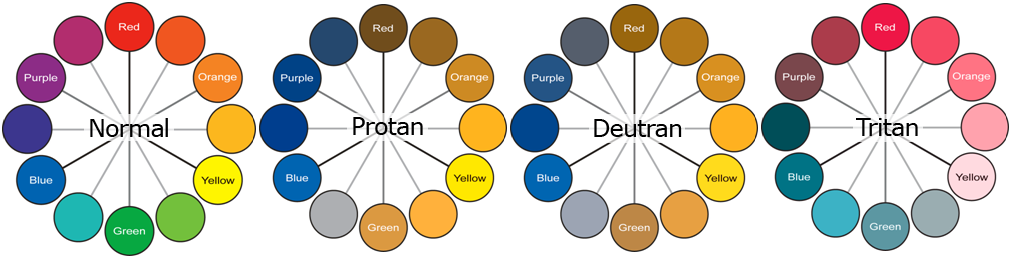
\includegraphics[width=0.9\textwidth]{images/background/ColorBlindnessCorrespondance.png}
    \caption[Correspondance of Colors Between Visual Deficiencies]{Correspondence of Colors Between Normal Vision,
    Protanopia, Deuteranopia and Tritanopia.\protect\footnotemark{}}
    \vspace{-10pt}
    \label{fig:correscolorblind}
\end{figure}
\footnotetext{"What About Color Blindness?", Available at: \url{www.bit.ly/1O7IK4G}. Last accessed on October 17th, 2016.}
%
\begin{wrapfigure}[10]{R}{0.25\textwidth}
	\centering
    \vspace{-\baselineskip}
    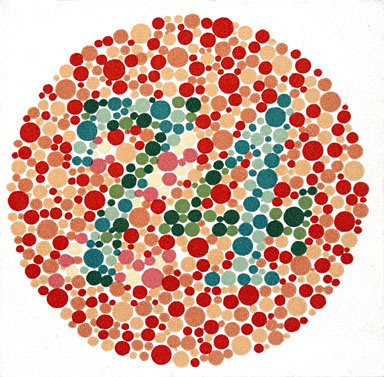
\includegraphics[width=0.25\textwidth]{images/background/IshiharaPlates.jpg}
    \caption[Pseudisochromatic Plate]{An example of a Pseudisochromatic plate.\protect\footnotemark{}}
    \label{fig:ishihara}
\end{wrapfigure}
\footnotetext{"Ishihara Color Test", Available at: \url{www.bit.ly/1jp3lm3}. Last accessed on October 17th, 2016.}
%
Color deficiency can be diagnosed through an eye examination. During that test, it will be used
specially designed figures composed with colored dots, called \textbf{Pseudisochromatic Plates}, which
include a number or a figure supposed to be easily decoded by someone without a visual deficiency, as the example
of the figure \ref{fig:ishihara}. The user is asked to look at the plate with the figure and distinguish
the number/figure: if it is correctly spotted the number, the subject does not have a particular type of deficiency; if some difficulty is found, that constitutes an evidence of possible color blindness. This test was created by Dr. Shinobu Ishihara in 1917: the original test
consisted of 38 plates, but later \cite{Ishihara1972}, the author published a
simplified version with 24 plates. This test has been used since then in various researches about color perception.
%
\subsubsection{Mental Models and Codes}
Whether agreeing or not on it as an intrinsic existing characteristic, we perceive color on every
subject we look at. In fact, one of the things you are taught by your relatives and educators is the concept of
painting with color pencils, gouaches or felt pens; mixing colors is a constant,
you naturally learn how colors are disposed in a color wheel and, in most of the case, a subtractive color
model like the \textbf{RYB} is taught. As Gosset \emph{et al.} state \cite{Gossett2004}, the usage or learning of
subtractive color spaces, in childhood, modifies the mental color model of each person. Typically, these models are quite
different from the \textbf{RGB} model, and this can create confusion to
the observer, since these types of models constitute additive color spaces. \par
Mental models help spreading color standards through the population and colors turn out to be instantaneously
recognized as information. For example, in 1968 Vienna Convention on Road Signs and Signals \cite{Nations1995}, it was standardized signing system for road traffic, from road signs and marks, to traffic lights;
this convention was created to increase road safety, by creating consistent common rules every country
should follow; other examples of color standards are the International Maritime Sinal Flags
\cite{Agency2003} (used on ships to transmit messages) or to electrical wiring conventions, among many others. \par
%
\begin{wrapfigure}[9]{R}{0.25\textwidth}
	\centering
    \vspace{-10pt}
    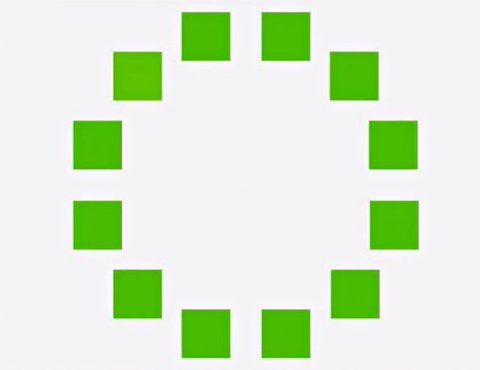
\includegraphics[width=0.25\textwidth]{images/background/Himba_green-color-ring.jpg}
    \caption[Himba Test: Green Color Ring]{Example of a Green Color Test made.\protect\footnotemark[8]}
    \label{fig:himba}
\end{wrapfigure}
%
Color is even perceptually different among different countries, continents, environments and genders:
as is know by now\footnote{"Where Man See White (...)", Available at:
\url{www.bit.ly/1AMHgcW}.
Last accessed on October 17th, 2016.} \cite{Ginter2011}, women can detect and describe with much more detail color than men, the
photoreceptors of men take a little longer wavelengths to perceive hue of a color; this question remain
to be fully researched, but the difference between genders is a certainty. In 2011, BBC shot a
documentary\footnote{\label{itsnoteasy}"It's Not Easy Seeing Green". Available at:
\url{www.nyti.ms/1S71yVo},
Last accessed on October 17th, 2016.} in which they explore the differences from the western color
perception, and tribal color perception; the researchers presented a circle of squares with different
shades of green (Figure \ref{fig:himba}), to the Himba tribe from Northern Namibia. Surprisingly, they were able to detect a larger
number of shades of green than a western, non-colorblind person: this may occur because their environment do not
manifest as much colors, and they need to detect different shades to hunt and pick up vegetation and
fruits, which traditional western communities do not need to do. \\
%
Every color is mapped into models which mathematically represent them, despite of physical attributes of display conditions.
All of these models are mapped against a \emph{Color Space} that maps the real-world colors in discrete values.
%
%%%%%%%%%%%%%%%%%%%%%%%%%%%%%%%%%%%COLOR MODELS AND SPACES%%%%%%%%%%%%%%%%%%%%%%%%%%%%%%%%%%%%%%%
%
\subsection{Color Models and Spaces}
\label{subsec:colormodelspaces}
%
\subsubsection{Colorimetry}
Mixing the three primary color light channels to match any color is no longer an oddity and it constitutes
the basics of \emph{Colorimetry}: it is the science used to quantify and describe the human perception of color.
We can describe color as the following equation \cite{Ware2012}:
\begin{equation}
C = sS + mM + lL
\end{equation}
%
\begin{wrapfigure}[9]{r}{0.25\textwidth}
	\centering
    \vspace{-15pt}
    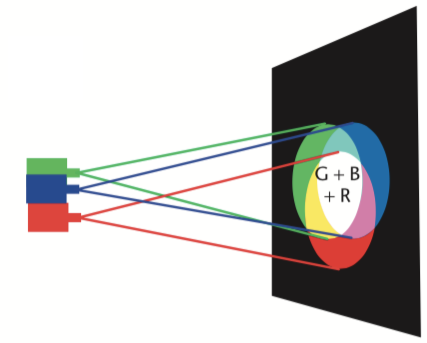
\includegraphics[width=0.25\textwidth]{images/background/Trichromacy.png}
	\caption[Trichromacy Theory]{Color-matching setup. \cite{Ware2012}}
\end{wrapfigure}
%
where C stands for the color to be matched, \emph{S, M} and \emph{L} are the primary light sources used to create the final
color and that are detected in three types of cones, \emph{s, m} and \emph{l} represent the precise amounts of each primary
lights. Not only by adjusting these primaries, but also by modifying their values, it becomes possible to
state any colored light, describing it as a weighted
sum of any three distinct primaries; this is the fundamental principle of colorimetry, the freedom to change from
one set of primaries to another, grounding the decision on phosphors of a monitor, a set of lamps or on the
sensitivities of the human cone receptors. Of course, this freedom comes with a price: it would be very difficult
do maintain and calibrate standardized lamps, specials instruments to evaluate color precision would be very
expensive and this would not be very practical. \par
To solve this, it was assumed that every human being had about the
same sensitivities to different colors (excluding the obvious color deficiencies), and the same receptor functions;
it was the time to start creating color specification standards and understand the principal concepts of it.
%
\subsubsection{Color Fundamental Concepts}
The organization and perceptual evaluation of color depends on some concepts which have been referred
before. They will be explained in this report, helping us understand how every color model and spaces work.
This concepts are listed below, with an appropriate explanation seeking them.
%
\begin{figure}[H]
  \centering
  \vspace{-10pt}
  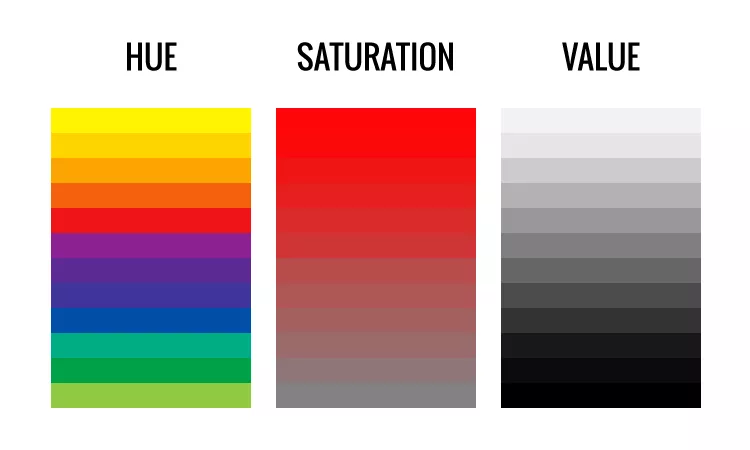
\includegraphics[width=0.5\textwidth]{images/background/Hue_Saturation_value.png}
  \caption[Hue, Saturation and Value Comparison]{Comparison between Hue, the concept of Saturation and Lightness (or Value).\protect\footnotemark{}}
  \vspace{-25pt}
  \label{fig:hsvconcepts}
\end{figure}
\footnotetext{"How to Analyze Data (...)", Available at: \url{www.bit.ly/1KHHtg2}. Last accessed on October 17th, 2016.}
%
\paragraph{\ul{Hue}} As defined in \textbf{CIE Color Appearance Model of 2002} \cite{Moroney2002}, hue is
“the degree to which a stimulus can be described as similar or different from stimuli that are described”
as red, green, blue, yellow, orange or violet. In case of two colors that are presented with the same hue, the
distinction is made using adjectives referring to their lightness or colorfulness. Also, it was created the
term \textbf{Unique Hue} to describe those colors that are instantaneously recognized as pure, the ones which do
not are the resulting product of a mixture; the colors known as unique are only four: Red, Green, Blue
and Yellow. The concept of Hue is represented in Figure \ref{fig:hsvconcepts}, on the left column.
%
\paragraph{\ul{Saturation}} This is a color term commonly used by imaging experts, to define a
range from \textbf{pure color (100\%) to gray (0\%)}; a pure color is fully saturated. From a perceptional
point of view, saturation influences the grade of vividness or purity of a subject: a desaturated image is
said to be dull or washed out, creating the impression of being softer. In other words, saturation is
determined by the combination between light intensity and its distribution across the spectrum; the purest
color is obtained with high-intensity wavelength and, as this wavelength drops, the saturation also drops
and the color turns into gray. For example, in Figure \ref{fig:hsvconcepts}, it can be seen
different saturation values for Red Color, varying from the purest red to gray. However, this concept must not be
confused with \textbf{Colorfulness} (which is the absolute color intensity of a light stimulus) and with
\textbf{Chroma} (which refers to the perceived strength of a surface color).
%
\paragraph{\ul{Lightness}} This concept is usually known as \textbf{Value} or \textbf{Tone}, and is related
to the variation of light in the subject, either lighter or darker (as seen on the right column of Figure
\ref{fig:hsvconcepts}): light colors are called \textbf{Tints} and dark colors are called \textbf{Shades}.
It defines the range from \textbf{dark (0\%) to fully illuminated
(100\%)} and judges the lightness of an illuminated area, compared to another area that appears to be white
or highly transmitting.
%
\paragraph{\ul{Brightness}} It is an attribute of our perception, highly influenced by color’s
lightness, but not to be confused with it! It is the perception of whether a subject is radiating or
reflecting light. For one color of a given hue, the perception of brightness is influenced by its saturation:
if we increase it, the color also looks brighter.
%
\begin{figure}[htbp]
  \centering
  \vspace{-5pt}
  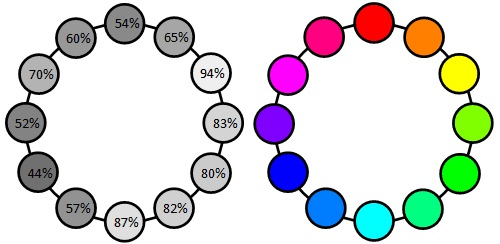
\includegraphics[width=0.45\linewidth]{images/background/Luminance.jpg}
  \caption[Luminance]{Luminance schematic.\protect\footnotemark{}}
  \vspace{-25pt}
  \label{fig:luminance}
\end{figure}
\footnotetext{"Color Luminance", Available at: \url{www.bit.ly/22O3vdp}. Last accessed on October 17th, 2016.}
%
\paragraph{\ul{Luminance}} It is a measurement of light, which assesses the luminous intensity
of a color. You can lighten or darken a color by adjusting its lightness value, but lightness is not the
only dimension to consider for luminance: that is because each hue has an individual luminance value; if
luminance is dependent on hue, it is also dependent on saturation; by reducing the saturation value of
any pure hue to 0\% results in a 50\% gray and 50\% value in luminance. For hues with natural luminance
above 50\%, the luminance decreases when saturation level decreases; contrary, if the luminance
is below 50\%, it will increase when the saturation level decreases. The Figure \ref{fig:luminance} describes
the percentage of white that each hue contains, being white the maximum percentage of 100\%.
%
\paragraph{\ul{Chromaticity}} Similarly to what happens with saturation, it is an objective
specification of the quality of a color, but regardless of its luminance. As it will be seen in a while, it
is what is shown in the CIE 1931 XYZ Color Space Diagram.
%
\paragraph{\ul{Contrast}} This concept estimates the influence of luminance that makes an object
distinguishable from a background. The Human Visual System determines contrast by the difference in the color
and brightness of the object and other subjects within the same field of view.
%
\paragraph{\ul{Temperature}} This is a characteristic of visible light with important applications
in lighting, photography and other areas. It is the temperature of an ideal black-body radiator (one which
absorbs all electromagnetic radiation that reaches it) which would radiate light of similar hue
to the radiating light source. Cool colors are the ones with temperature over 5000 Kelvin (K), conveying a
bluish white color; warm colors have temperature around 2700 K to 3000 K. For example, the light emitted by
a candle flame has a temperature of 1850 K and an orangish color, opposite to the color temperature of a
clear blue sky, which temperature goes around 15200 to 27000 K. \\ \par
%
Being the most relevant concepts of color introduced, it is time we start establishing relationships between
them: this type of relationships are created and reflected in color spaces and models, typically with three or
four color components. There is a fairly generous amount of them, but only a portion of these are interesting to
our research.
%
\subsubsection{Defining Color Models}		%% COLOR MODELS
%
The concepts of \emph{Color Spaces} and \emph{Color Models} are often confused but, in fact, they do not present the same idea
(although they do use similar conceptions). Color models exist to mathematically conceive a description of color,
in which color spaces will be based and present the equivalent colors. It is relevant to settle a distinction among
them, paying special attention to the fundamental \emph{CIE Color Space}, which is acquired as one of the most
fundamental perception studies. \par
%
A color model is a mathematical description of color, which is substantively different from a color space: the latter represents
the gamut of colors described accordingly to the primitives of a color model, containing not only visible colors
but also colors that are impossible to represent on physical devices. \par
There are two types of color models: additive and subtractive. \textbf{Additive Color Models} use light
to display color mixing, mixing primary colors such as Red, Green and Blue; equally combined and
overlapped, they form white light, whereas \textbf{Subtractive Color Models} mix colors using paint pigments
and the result of any mix is a color that tend to be darker, the more you mix it. Additive models are used
in computer graphic displays, while subtractive models are commonly associated to dyes and inks. Examples
of this color models are given below \cite{Ware2012}. \par
%
\begin{wrapfigure}[9]{r}{0.25\textwidth}
  \centering
  \vspace{-10pt}
  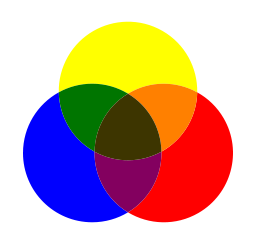
\includegraphics[width=\linewidth]{images/background/RYB.png}
  \caption[RYB Color Model Schematic]{RYB Model.\protect\footnotemark{}}
  \label{fig:RYB}
\end{wrapfigure}
\footnotetext{"RYB Plano", Available at: \url{www.bit.ly/22MHzPJ}. Last accessed on October 17th, 2016.}
%
\paragraph{\ul{RYB}} One of the first models to appear was the RYB color model, an
abbreviation for \ul{Red-Yellow-Blue}, created in the late 16th century by Franciscus Aguilonius
in the belief of having a set of colors capable of creating all other colors, when mixed. This theory
was considered a standard almost for two entire centuries: even Newton used it on his famous work
“Optiks” (1706) about light refraction and diffraction, creating a color wheel which represents the
relations among colors. In the beginning of the 18th century, the RYB
model served as the base to fundamental studies about color vision: the german poet Joan Wolfgang
von Goethe, published a relevant work about his visions on the nature of colors and how they are
perceived by humans under different circumstances; his work was widely accepted between philosophers,
since its analysis was more focused on the human perception of color and not so much on the analytic
specification of color. \\
This color model is a \textbf{subtractive color mixing model}, in which the primary colors are Red,
Yellow and Blue, and the secondary colors are Orange, Purple and Green. However, this model was quite
limited in what was concerned about color perception and it was necessary to specify a new model which
would create a standard in representation of images on digital display devices. \par
%
\begin{wrapfigure}[9]{r}{0.25\textwidth}
	\centering
	\vspace{-10pt}
	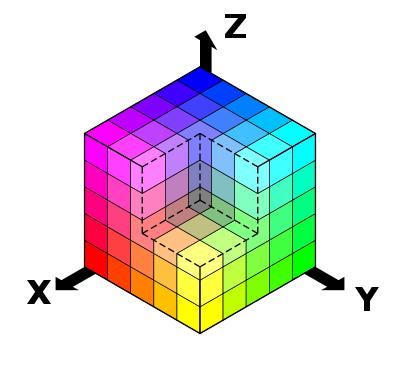
\includegraphics[width=\linewidth]{images/background/RGB.png}
	\caption[RGB Color Model Schematic]{RGB Model.\protect\footnotemark{}}
	\label{fig:RGB}
\end{wrapfigure}
\footnotetext{"RGB Cube", Available at: \url{www.bit.ly/1n5QCdZ}. Last accessed on October 17th, 2016.}
%
\paragraph{\ul{RGB}} Subsequently, the RGB color model stood out as an additive
model in which \ul{Red-Green-Blue} colors were mixed together to produce a wide field of colors;
the RGB model is closer to the way human vision encodes images. When combined, red and green light rays
produce yellow, red and blue produce magenta (or purple) and blue and green produce cyan. For example,
this color model is used in Cathode Ray Tube monitors, flat-panel displays, video projectors and
light systems in theater; this characterizes this model as a device-dependent color model. When all
three primary color channels are 0 percent, the result is black color. If all three primaries are 100
percent of its intensity, the result is white. This color model is represented as three dimensional cube,
with each corner being the purest colors, as in the Figure \ref{fig:RGB}.
Nonetheless, this color model needed improvements, specially a better geometrical representation, since RGB does not create
an accurate match to the color mixture recognized by human vision.
%
\begin{wrapfigure}[6]{r}{0.35\textwidth}
	\centering
	\vspace{-10pt}
	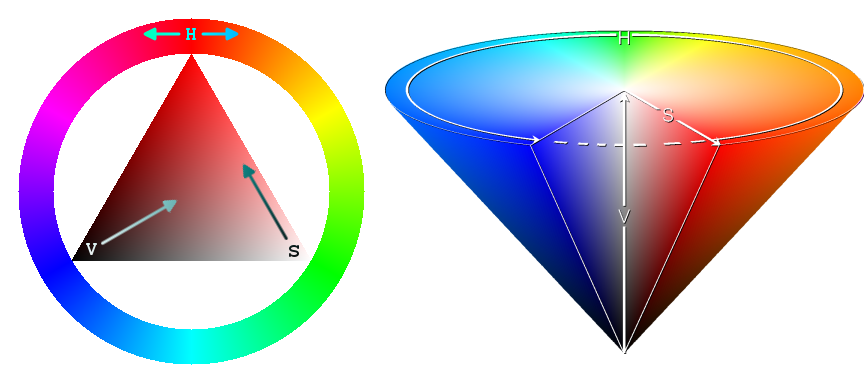
\includegraphics[width=\linewidth]{images/background/HSV_TriangleCone.png}
	\caption[HSV Triangle and Cone Representation]{HSV Model.\protect\footnotemark{}}
	\label{fig:HSV}
\end{wrapfigure}
\footnotetext{"Computer Graphics (CS 4300) (...)", Available at: \url{www.bit.ly/1OQh8Vh}. Last accessed on October 17th, 2016.}
%
\paragraph{\ul{HSV and HSL}} The HSV model was developed to correct the flaw in RGB. This acronym
stands for \ul{Hue-Saturation-Value}, depicting a three-dimensional color model: it aims to
present relationships between colors, which is a direct improvement from RGB. There are several
geometrical representations of this model, from cones to cylinders, but all of them provide the same
visualization and concept disposal: Red, Green, Blue, Magenta, Yellow and Cyan \ul{Hues} are equally
disposed in a circumference of a circle composing the color wheel, (you can think of it as a cut of the cylinder, or the cone base)
with the white color in the center; from the center of the circle towards the outer edge, varies the
\ul{Saturation} of colors, being the most saturated the farthest position from the center. In a
perpendicular edge departing from the center of the circle until the bottom of the cylinder/cone, it
oscillates the \ul{Value}, being the bottom value equal to 0 and the darkest color (black), the lightest
color (white) on top and, in-between, colors vary its darkness. The perception of relevant color
proximity that this model brings is counter-posed by the lack of perceptual uniformity. \\
It was proposed a parallel model to HSV, which was called \textbf{HSL} due to its resemblance to the
first. The main difference of this model lays on the last color component used, which is
\ul{Lightness}. Here, the value’s axis is substituted by lightness, which in this case makes
the bottom completely black and the highest plane completely white; a very common representation of HSL
is the bicone or a cylinder. Both HSV and HSL are examples of \textbf{additive color models}. \par
%
\begin{wrapfigure}[10]{r}{0.27\textwidth}
	\centering
	\vspace{-10pt}
	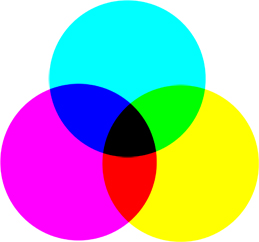
\includegraphics[width=\linewidth]{images/background/CMYK.jpg}
	\caption[CMYK Color Model Representation]{CMYK Model.\protect\footnotemark{}}
	\label{fig:CMYK}
\end{wrapfigure}
%
\paragraph{\ul{CMYK}} CMYK works as a subtractive color model, with four color
components, and is primarily used in printing industries, given the feature of printed ink of reducing
the light that otherwise would be reflected. It is composed by four color: \ul{Cyan-Magenta-Yellow-Key}.
Key value is representing the black color, which is used because the combination of the three primaries
does not produce a fully saturated black color. This color model is able to produce the entire color
spectrum of visible colors, due to the \textbf{half-toning} process it executes: tiny dots of each
primary color, with an assigned saturation, are printed in a pattern small enough so it is perceived
as a solid color. This process allows the printing of more than seven colors, the
amount of possible mixture combinations which could be created if the primary colors were printed as
a solid block of color. In order to improve the print quality and reduce moiré patterns, the screen
for each color is set at a different angle. \\
This color model may be viewed as the inverse of RGB color space, since it represent all the colors
produce by the mixture of RGB colors: Green-Blue produce Cyan, Red-Blue produce Magenta and Red-Green
produce Yellow. CMYK is a device-dependent space. \par
\footnotetext{"What is the difference (...)", Available at: \url{www.bit.ly/1Ohu0lp}. Last accessed on October 17th, 2016.}
%
\subsubsection{Defining Color Spaces}			%% COLOR SPACES
%
A color space is the set of colors originated by the specification of a mathematical model of primitives; it also
allows the representation of reproducible colors on a given physical device. It relates the description
of a color model to actual colors, being a three dimensional object that contains all realizable color
combinations. They can be, generally, grouped onto three categories:
%
\begin{enumerate}
	\setlength\itemsep{0.01em}
	\item \textbf{Device-Dependent Spaces}, which express color relative to some other reference space. It
	  indicates the subset of colors which can be displayed using a particular device (\emph{e.g.} a monitor or a
	  printer) or captured by a recording device.
	\item \textbf{Device-Independent Spaces}, which express color in absolute terms, serving as universal
	  reference colors.
	\item \textbf{Working Spaces}, used by image editing software and file formats to constrain the range of
  	colors to a standardized palette. For example, one of the most used color working space is Adobe RGB 1998.
\end{enumerate} \par
%
There were two relevant studies made about color spaces: the fist one is the \textbf{Munsell Color System},
which had began in 1898 and saw its full expression in 1905; the second is one of the principal color spaces used to describe the
entire range of human perceivable colors, which is the \textbf{CIE Color System}. The CIE space of visible color is expressed
according to different components: \textbf{CIE 1931 XYZ, CIE-L*a*b* and CIE-L*u*v*}, and all three present the same range of colors.
%
\begin{wrapfigure}[10]{R}{0.25\textwidth}
  \centering
  \vspace{-\baselineskip}
  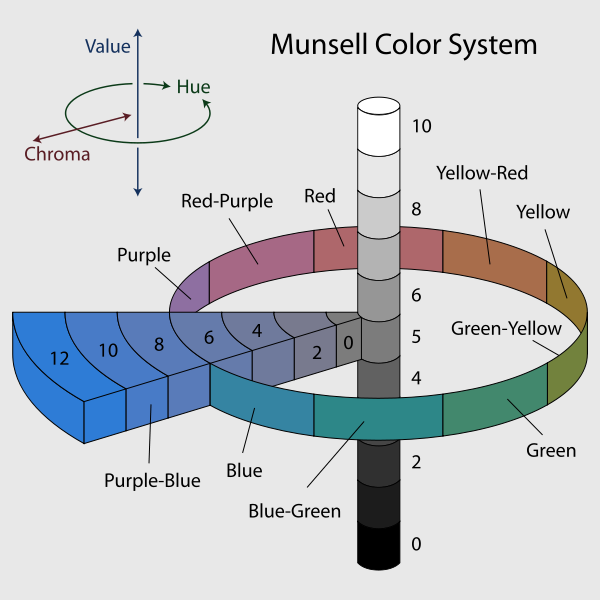
\includegraphics[width=\linewidth]{images/background/MunsellSystem.png}
  \caption[Munsell Color System Representation]{Munsell Color System.\protect\footnotemark{}}
  \label{fig:munsell}
\end{wrapfigure}
\footnotetext{"Munsell Color System", Available at: \url{www.bit.ly/1mJsH3I}. Last accessed on October 17th, 2016.}
%
\paragraph{\ul{Munsell Color System}} One interesting color system is the one created by
Professor Albert H. Munsell in the first decade of the 20th century \cite{Munsell1919}. This was the first system to separate
hue, value and chroma into perceptually different dimensions, and also illustrate in a systematic way these
components in a three dimensional space. It consists of a cylindrical color solid, where value is measured
vertically from 0 (black) to 10 (white), hue is measured in degrees around horizontal circles and chroma,
radially measured in concentric circles. \\
Each circle of the cylinder is divided into five principal hues: Red, Yellow, Green, Blue and Purple, where
intermediate hues can be found
in-between the principal ones. Two colors with equal chroma and value - residing in the same circle - but
found on opposite sides are complementary colors, and create gray color found in center of the
circle, when mixed together.  Colors in this system are defined in the format \textbf{“H V/C”}, for example,
“5R 5/10” means Red Hue, with 5 meaning middle value and a chroma of 10, indicating a high level of purity. \par
%
\paragraph{\ul{CIE 1931}} The \emph{Commission Internationale de l’Éclairage} (\textbf{CIE}, or
International Commission on Illumination) defined in 1931 the first set of color spaces, which defined the
mapping between physical pure colors and standard observer measurements of perceived color: they are,
nowadays, identified as the \textbf{CIE 1931 Color Spaces}, and can be disjointed onto two spaces: the
\textbf{CIE 1931 RGB Color Space} and the \textbf{CIE 1931 XYZ Color Space}. Remembering Section \ref{sec:humaneye},
we discussed the existence of three types of cones, S, M and L, which correspond to three different types
of cone stimulation; the CIE color space maps the range of physically produced colors to a description of color
sensations registered by the observer, which come in terms of \emph{tristimulus values}: this system uses
a set of abstract primaries abstracted to XYZ, chosen for their mathematical properties (instead of SML
\emph{stimuli}) which will cast the color perception into this new coordinate system.
The \textbf{CIE XYZ} comprises all color sensations a human can perceive, standing out as a standard for
other color spaces and the tristimulus values have the following properties:
%
\begin{itemize}
	\setlength\itemsep{0.01em}
	\item All tristimulus are positive for all color. The XYZ axes are purely abstract, but all perceived
	colors fall within CIE gamut \emph{i.e.} complete subset of colors.
	\item The X and Z values have zero luminance, being the Y value the only one which represents luminance
	information. By defining this, CIE space allows the XZ plane to contain all possible chromaticities
	(a specification of a color, regardless of luminance) at a given Y luminance.
\end{itemize} \par
%
\begin{figure}[htbp]
  \centering
  \vspace{-15pt}
  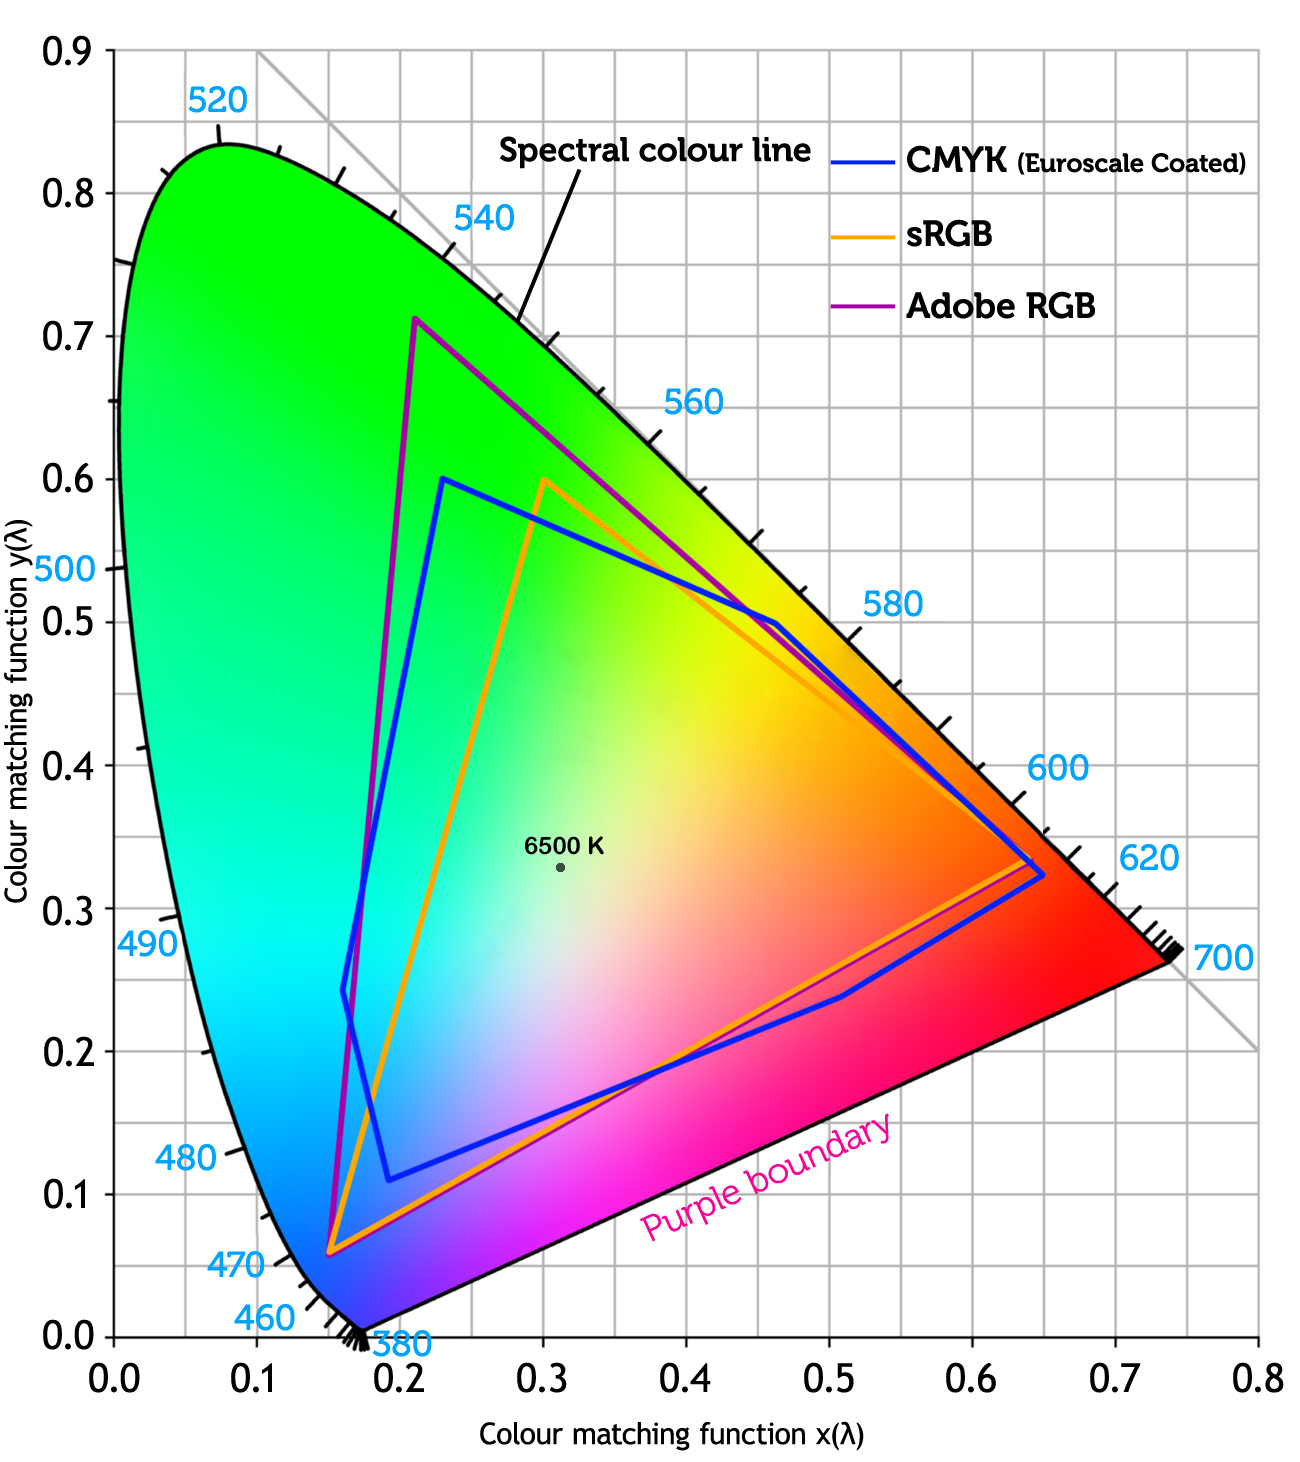
\includegraphics[width=0.35\textwidth]{images/background/CIE_RGB_CMYK.jpg}
  \caption[CIE Horseshoe with AdobeRGB, sRGB and CMYK Gamuts]{CIE Color Diagram, with CMYK, sRGB and AdobeRGB Color Gamuts depicted.\protect\footnotemark{}}
  \vspace{-10pt}
  \label{fig:cie}
\end{figure}
\footnotetext{"CMYK Colour Model/Colour Space", Available at: \url{www.bit.ly/1TIo5pd}. Last accessed on October 17th, 2016.}
%
The CIE 1931 color diagram, as seen on the Figure \ref{fig:cie}, represents all the chromaticities visible to an average
person, called the gamut of human vision., in particular several subsequent RGB color spaces, such as the \textbf{sRGB}
(the most commonly used RGB space, in media devices), the \textbf{Adobe RGB and Apple RGB} which define their own
particular gamut of colors. It has a 3D shape, but the most recognized form is a 2D plane, with a
horseshoe shape, due to its curved edge that represents the edge of human perceivable colors, also known as the
spectrum locus; on the bottom of the graph, a
straight edge can be seen and it goes by the name of line of purples (or Purple Boundary), going from red to violet. All of this
edges are considered to be the only fully saturated colors. The \textbf{chromaticity diagram} has some
interesting properties \cite{Ware2012}:
%
\begin{itemize}
	\setlength\itemsep{0.01em}
  \item If two colored lights are represented by two points in the diagram, the resultant color of those
  two points’ mixture will always lie on a straight line between them.
  \item Any set of 3 light specifies a triangle in the diagram: each corner represents a different light
  source. Any color within this triangle can be created by a mixture of those three lights.
  \item CIE defines a standard for white light illumination: it specifies a number corresponding to
  different kinds of daylight. The most commonly used is \textbf{D65}, chromaticity coordinates being: $x = 0.313 , y = 0.329$.
  To contrast, \textbf{Illuminant A} (an incandescent tungsten light source) has coordinates: $x = 0.448 , y = 0.407$,
  which is considerably more yellow than normal daylight.
  \item The vividness of a color is defined by the excitation purity, which quantifies
  distance along a line between a particular pure spectral wavelength and the white point of the diagram.
\end{itemize} \par
%
The CIE Color System is both a Color Model and a Color Space since, at the same time, it describes
a mathematical representation using XYZ primaries and represents the superset of the entire range of human
perceivable colors. The \textbf{CIE RGB Color Space} is one of the many subsets of CIE XYZ. \par
%
\paragraph{\underline{CIE-L*a*b}} It is a device-independent color space based on color-opponent axis,
created in 1976. The two axis are represented by the \textbf{a*} and \textbf{b*}, where the first one represents the
Red-Green axis and the latter the Blue-Yellow one; the \textbf{L*} variable represents the lightness. This
color space is often used when graphics have to be printed and converted from RGB to CMYK color model, as
L*a*b* space contains both color gamuts. \par
There are some particularities related to this space: \textbf{i)} The values for the
three variables are absolute, with a pre-defined range; \textbf{ii)} L* = 0 represents black and L* = 100 the brightest white;
\textbf{iii)} As for the a* and b*, they will represent a neutral gray value at 0 value; \textbf{iv)} On the Red-Green Axis,
represented by a*, the positive end a* being the Red component and the negative end the Green component; \textbf{v)}
On the Blue-Yellow Axis, represented by b*, the positive end b* being the Yellow component and the negative end the Blue component;
 and finally, \textbf{vi)} The value limits are implementation-dependent, since they can vary between -100 and +100 or -128 and +127. \par
This color space derived into a cubic color space representation, which is recognized as the
\textbf{CIE-L*C*h*}, where the Cartesian coordinates of a* and b* are substituted cylindrical coordinates
\textbf{C* and h*}: the first one stands for \textbf{Chroma} and the second one for the angle of the
\textbf{Hue} in CIE-L*a*b* color wheel. \par
%
\subsubsection{Color Calibration}
%
The accuracy of color is critical in design: the color you see on a monitor, sometimes, is not what will appear on a printed sheet. The aim of calibrating a color is to adjust the color response of a device, establishing
a relationship to a standard color space or model. This represents an important step when performing a
color perception research, since perception of a color is influenced by the light sources incident in the
device, the color space used by the device and the existent calibrated color of it. There are numerous
ways to perform a calibration of color, either by software or hardware: for example, there are colorimeters, which
are physical devices which can be placed close to the device screen and will stimulate individually every pixel
according to a concrete color setup, defined by the user. \par
%
\begin{wrapfigure}[9]{R}{0.4\textwidth}
	\centering
    \vspace{-10pt}
    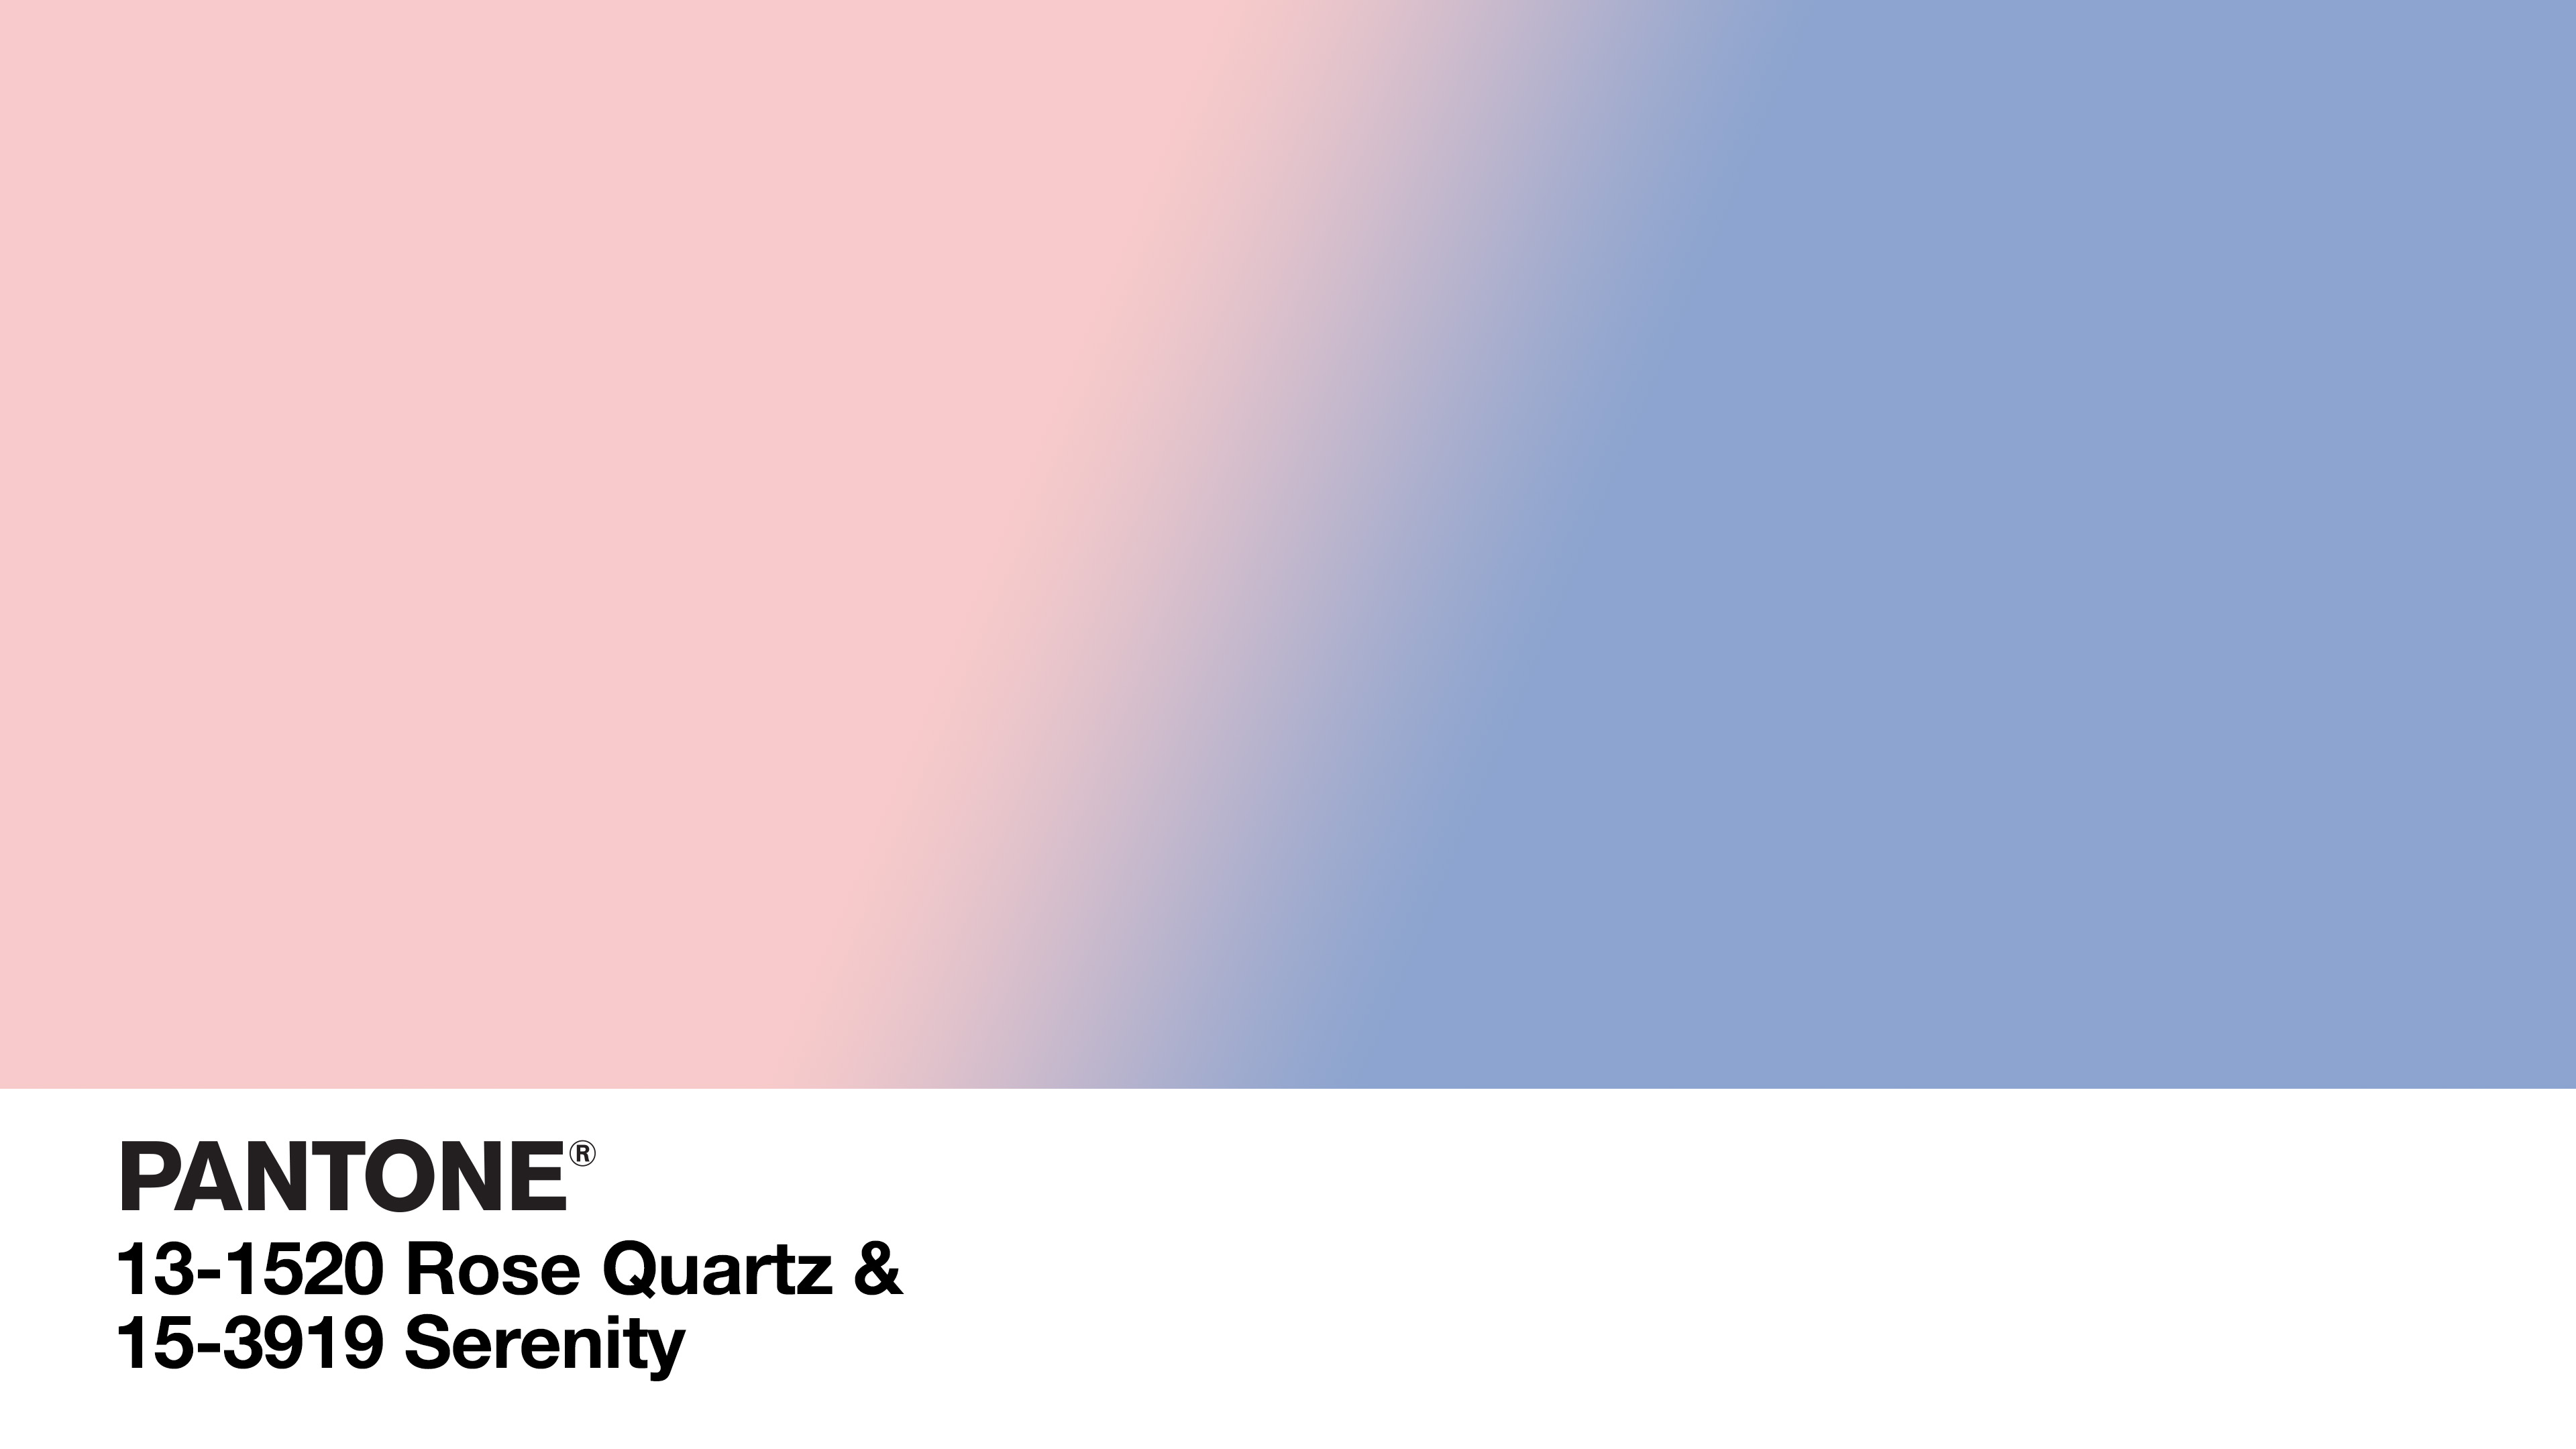
\includegraphics[width=0.4\textwidth]{images/background/Pantone_rose_serenity.jpg}
    \caption[Pantone Matching System - Marsala]{Pantone's Color of the Year.\protect\footnotemark[18]}
    \label{fig:pantone}
\end{wrapfigure}
%
Nonetheless, calibration standards were created to ensure the color correctness and expectation. The
\textbf{Pantone Matching System (PMS)} is a commercial standardized color reproduction system; by creating
this standard, printers and manufacturers around the world can refer to a specific Pantone color code to
make sure colors match with no doubt (as in Figure \ref{fig:pantone}). The PMS is recognized also, by the printing of a small catalogue with
a large number of small sheets which contain every possible Pantone color, in every tint or shade. The type
of paper used will affect the appearance of colors: Pantone covers this problem by showing how desired
color will look on coated, uncoated or matte paper\footnote{"The Pantone Matching System\textsuperscript{\textregistered}",
Available at: \url {bit.ly/1ZdsYNU}. Last accessed on October 17th, 2016.}.
PMS is used in a variety of industries, primarily offset printing. \par
%
Another commonly used standard is the \textbf{Natural Color System (NCS)},  based on the color opponent
axis description: there exist three pairs of opponent colors, the White-Black, Green-Red and Yellow-Blue,
which were introduced by Ewald Hering \cite{Ware2012}. The NCS is based in mechanisms involved in signal processing
in the ganglion cells in retina, which orientates the light to retinal cones before it is sent to the brain;
this is different from what happens with RGB, where information is acquired at low level on the cones and
rods. This color system is based on the six elementary colors referred in the beginning of the paragraph;
colors in NCS are defined by three values, specifying the amount of \textbf{darkness, the chromaticity and a
percentage value between two of the colors}. The intuit of this color system is
create color codes that can be spread and understood across the world. To define a color in this color
system you need to\footnote{\label{ncshowto}"How To Comunicate Your Color.", Available at: \url {bit.ly/1OSrttr}. Last accessed on Jauary 8th, 2016.}:
%
\begin{enumerate}
	\setlength\itemsep{0.01em}
	\item Identify the closest matching color area in the NCS Color Circle, which will give the family name
    of that color, the hue.
	\item Find you shade or tint in the color triangle of the color chosen in the first step. This will give
    you its darkness and chromaticity, which must add up to 100\%: if a percentage value remains, it is
    attributed to whiteness.
	\item Write the full name, preceding with “NCS”, adding “S” if the color is an NCS standard color.
\end{enumerate} \par
%
For example, \textbf{NCS S 1070-Y10R} translates into a NCS standard color perceive as: 90\% Yellow and
10\% Red, with 10\% of Whiteness and 70\% of Chromaticity value. Since 10\% + 70\% = 80\%, the remaining
20\% belongs to \emph{Whiteness}.
%
\subsubsection{Color Scales}
%
\begin{wrapfigure}[10]{r}{0.3\textwidth}
	\centering
    \vspace{-10pt}
    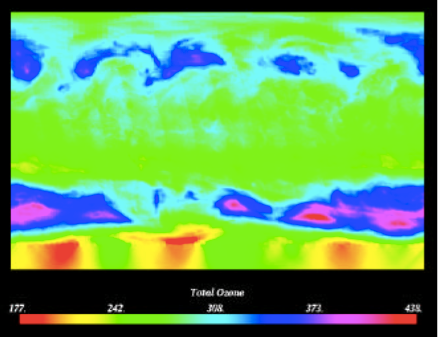
\includegraphics[width=0.3\textwidth]{images/background/SpectrumScale.png}
    \caption[Spectrum Scale Example]{Spectrum Scale. \protect\cite{Rheingans2000}}
    \label{fig:spectrum}
\end{wrapfigure}
%
Color is commonly used in data visualization in order to convey various types of information. It is derived into color scales,
which are pictorial representations of a set of numerical or categorical values, with every value having
a matching color; by attributing different colors to different values, we can create a gradient of colors
which eventually transmits continuity and the idea of perceptual steps. Penny Rheingans \cite{Rheingans2000} surveyed some
common (and not common) techniques for color scales used to present univariate and bivariate data. \par
%
For Single-Variable Color Scales, a \textbf{Saturation Scale} can be created by keeping the hue
invariable, oscillate the color saturation; the biggest advantage is the simplicity and its intuitiveness,
the biggest disadvantage the low PDR (Perceived Dynamic Range). Also, \textbf{Spectrum Scale} (Figure \ref{fig:spectrum})
is a very commonly used scale, keeping the saturation and brightness invariables, oscillate hue within its full
range (from red, orange and yellow, to yellow, green, blue and then purple). The problem lies in the fact that this scale
is not intuitively continuously perceived for all observers\footnote{"Dear NASA (...)",
Available at: \url{www.blog.visual.ly/rainbow-color-scales/}. Last accessed on October 17th, 2016.}:
perceptual discontinuities occur in the scale in the transitions between primary colors, in the “naming boundaries”
of each color (the boundaries of primary colors that can be described and named by the observer), which can mislead the
observer and make him perceive limits where they don’t exist. For a protanopic person, rainbow color scales
appear to have repetitive colors. Also, there are colors that appear brighter than
others, for example yellow, since it activates both M and L Cones (Green and Green-Red, respectively), creating
the false expectation of a greater value associated to yellow. \par
%
\begin{wrapfigure}[10]{R}{0.3\textwidth}
	\centering
    \vspace{-10pt}
    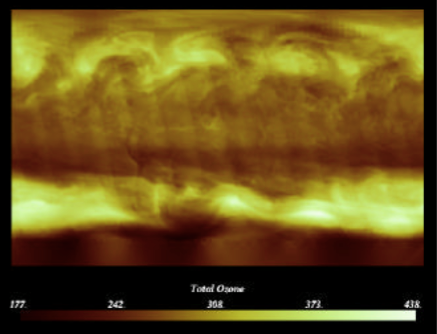
\includegraphics[width=0.3\textwidth]{images/background/HeatedObjectScale.png}
    \caption[Heated-Object Scale Example]{Heated-Object Scale. \protect\cite{Rheingans2000}}
    \label{fig:heatedobject}
\end{wrapfigure}
%
Sometimes, as Levkowitz explained \cite{Levkowitz1996}, the \textbf{Gray Scale} is the most used,
being black the lowest value and white the highest value: its advantage is the efficiency for the human
visual system; however, it has a limited PDR and, combined with aesthetic reasons, people tend to seek
alternative color scales. \textbf{Heated-object Scale} (Figure \ref{fig:heatedobject}) is also very
common, by combining gray scale and
spectrum scale, it augments monotonically with luminance; it fluctuates from black, to red, orange to yellow
and, in the end, to white. It happens to have more distinguishable perceptual steps and more contrast, than
the gray scale. \par
%
Rheingans defines \textbf{Hue-Other Scales} for two or more variables, as mapping variables to
different color models, like hue, lightness or saturation. Lightness
gives the perception of order, as we perceive the values as having a natural order. It is also easier to
judge the relative magnitude of two lightness values than of two hues. For example, areas with similar hue
values, but differing lightness, are easier perceivable as related than areas with similar lightness, but
different hue.
%
%%%%%%%%%%%%%%%%%%%%%%%%%%%%%%%%%%%%%%%% COLOR BLENDING - RELATED WORK %%%%%%%%%%%%%%%%%%%%%%%%%%%%%%%%%%%%%%%%%%%%%
\section{Related Work}
\label{sec:related_work}
%
Color plays an important role on how we perceive subjects and in the information we extract from them; it is usually
associated to the representation of information, due to is expressiveness and the familiarity that users have: if you
picture a graph or a chart, you instantaneously think of colors to represent variables. \par
%
Visualizing information is a task which, at the same time, communicates information and alleviates
cognitive load associated with data interpretation. Usually, when it comes to encoding information, color
appears as the number one choice, due to the its ease of perception and familiarity. When representing
more than one colored variable at the same time, it would be useful to perceive interrelations among
them and if the users are able to understand which of these entities are related, or blended: this leads
us to the idea of blending colors together to form a mixture, conveying more than one channel of information.
Research has been made to conclude if people can distinguish different percentages of blended colors or
associate colors to daily-basis tasks, \emph{e.g.} reading and receiving emails \cite{Gama20143}. \par
On the other hand, researchers have been developing alternatives to color mixture, enabling the end users
to create different perspectives on how color is related; as we are going to see, color blending has its
features and flaws, which complementary techniques try to recover. \par
%
In this section of the Background, we focus the attention on work previously developed in this research field. We
start by analyzing the investigation conducted before, following it by an analysis of other user color studies
which were performed across the internet, since this subject will be important to define how we drafted our own
user study.
%
\subsection{Color Blending Research and Techniques}
\label{subsec:colorblending}
%
Until the year 2014, some aspects remained to be studied. Gama and Gonçalves started their research \cite{Gama20141}
aiming to study to which extent people are able to, given a specific color resulting from a mixture of
two colors, understand the blended color’s origin; besides, they studied which is the color model that
yields the most accurate results: hardware-oriented color models like RGB or color-printing models such
as CMYK, fail to provide a color perception description, unlike HSV. This pitfall is amended by CIE-L*C*h*,
by creating a perceptually uniform scale to lightness.  \par
%
\subsubsection{Data Visualization}
\label{subsubsec:datavisualization}
%
\begin{wrapfigure}[8]{r}{0.35\textwidth}
	\centering
    \vspace{-15pt}
    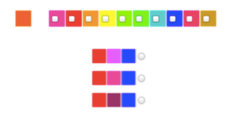
\includegraphics[width=0.35\textwidth]{images/background/TestDataVis.png}
    \caption[Color Blending for Data Visualization]{Example of Color Set. \protect\cite{Gama20141}}
    \label{fig:datavis}
\end{wrapfigure}
%
A user-study was designed \cite{Gama20141} to assess the afore mentioned goals, two sets of colors were created
from the model CIE-L*C*h*. The first (set A) had to do with dyadic mixtures, with pairwise combinations between
the four main colors (R: Red, G: Green, B: Blue, Y: Yellow): RG, RB, RY, GY and BY. The second set (set B) consisted
of triadic mixtures of the referred colors:
RRG, RGG, RBG, RYG, RRB, RBB, RYB, RYR, RYY, GBG, GBB, GYB, GYG, GYY, BYB and BYY. The study started with a
profiling questionnaire about the users; on the second part, a color blindness detection test was conducted
with a simplified 6-plate colorblindness Ishihara Test. On a third part, users were randomly
presented with a color from set A or B and were asked to chose from a color palette, the colors which mix
into that color, as in the top image on Figure \ref{fig:datavis}. After, users were presented to colors blended
into HSV, CMYK and CIE-L*C*h* and they had to pick the most natural transitions (bottom image of \ref{fig:datavis}).
The final step was a simple satisfaction questionnaire where users were asked to indicate in a 5-point Likert Scale,
how easy it was to find which pairs resulted in the colors given and the most natural blending option. \par
%
The study was performed to 73 non-colorblind, mostly middle-aged, all graduated users; the majority
(about 64\%) was male users and most everyone (96\%) lived in Europe. For the set A, the success rates
were higher for RY and GY color mixtures, which correspond to smaller angles in the CIE-L*C*h* color wheel,
and the worst success rates were consequently to wider angles in the wheel: BY, RG e RB.
Respecting set B, results were considerably lower which can indicate that either choosing few colors from
a wide palette is confusing or users were not able to correctly perceive the original colors which originated
the mixed color; however, the highest and worst rate of success is aligned with the set A, since GYG, GYY
and RYY yielded the best results, RRG, RBG, BYB and BYY the worst. Regarding, the most natural transition,
users chose CMYK as having the smoothest one, followed by CIE-L*C*h* and HSV; despite users attributed to
CIE-L*C*h* the second position in natural transition’s podium, they found it hard to perceive the colors
that were mixed during the study (which were mixed in this model). \par
%
The fact that CMYK has the smoothest transition to users is related to what Gosset \cite{Gossett2004} stated, that
subtractive color models learned in childhood restricts the mental model of color which users create;
in depth research has to be done to compare blending perception between CIE-L*C*h* and CMYK models. It
should also be take into consideration that, although the sample is large, there is a considerable gap
between genders: more women should be included in the study since, as previously mentioned, women can
distinguish a larger variety of shades. There is not an extensive cultural representation, just as there
is no representation of various educational levels besides graduated users, which could be interesting to show. \par
%
\subsubsection{Perception of Relative Amounts of Color}
\label{subsubsec:perception_amounts}
%
\begin{wrapfigure}[13]{R}{0.15\textwidth}
	\centering
    \vspace{-15pt}
    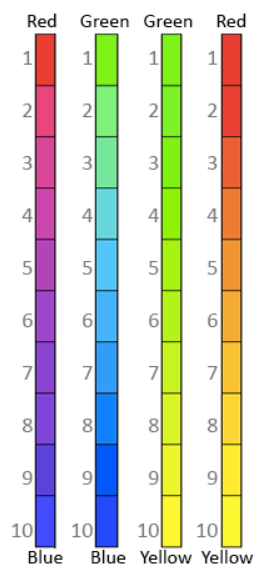
\includegraphics[width=0.15\textwidth]{images/background/TotalAmount.png}
    \caption[Perception of Relative Amounts of Color - Rulers]{10 Step Scales.
    \protect\cite{Gama20142}}
    \label{fig:amount1}
\end{wrapfigure}
%
Humans can perceive the original
components that created a particular color: the final study performed by Gama and Gonçalves relating Color Blending
Perception investigated precisely, the extent people can perceive relative amounts of color components in
blended colors \cite{Gama20142}. However, the amount of each component may not be evident: as it has been said before,
there are pairs of colors which yield better results than others due to cultural standards, conceptual models
or simply color conception. This has one major handicap: though reducing the cognitive load by
associating colors to information, it may not show the expected accuracy if we do not understand
human color perception. \par
%
To fulfill this problem, it was designed a user-study similar to the previous ones, consisting of a first
profiling phase, a color evaluation step and a 5-point Likert Scale to describe how easy it was to decide
the amount of each color component in the given color. Respecting the color evaluation step, it was created
a set of 10 interpolated colors for 4 pairs: (Red-Yellow), (Green-Yellow), (Green-Blue) and (Red-Blue),
as seen on Figure \ref{fig:amount1}. Then, users were presented with each of the 40 blended colors individually and
asked to rate these from 1 (only the first color component) to 10 (only the second color component). \par
%
20 participants have attended the study, equally divided by genders, non-colorblind and all european
citizens residing in Europe. Users happen to perceive most colors correctly regarding the pair (Red-Yellow)
and likewise colors in both extremes, even for other pairs: “central colors” are generally the most
problematic. An important conclusion from this research is that it should be considered, at maximum, 5
colors when blending colors, so that the relative amount of each color component is perceivable by the
users. Results have shown, also, that subjects found it moderately easy to perceive color component
weight in blended colors. \par
%
This study provides us several rules of thumb for crafting an information visualization or a color
blending perception: when the idea is to provide rough information, color information may be successfully
used; be that as it may, no more than three interpolations must be done between color pairs, so humans
can distinguish different component weights. Hence, a set of 5 colors is the optimal solution: 2
pairwise colors and 3 interpolations. \par
%
\subsubsection{Other Research}
\label{subsubsec:other_research}
%
\begin{wrapfigure}[11]{r}{0.4\textwidth}
	\centering
    \vspace{-10pt}
    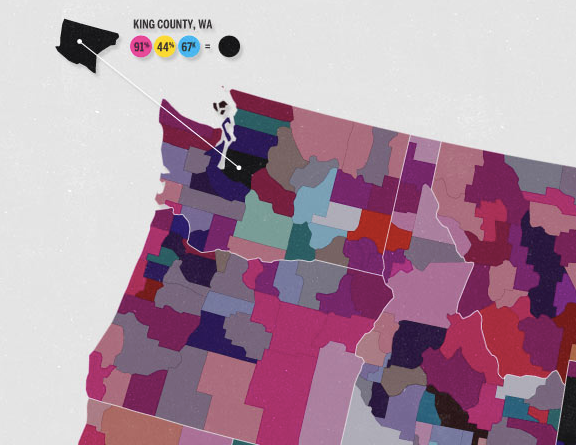
\includegraphics[width=0.4\textwidth]{images/background/CMYKbad.png}
    \caption[Color Blending: CMYK Bad Example]{Bad Color Blending Usage.\protect\footnotemark[25]}
    \label{fig:cmykbad}
\end{wrapfigure}
%
Apart from the previous referred studies, it is possible to give some
examples of current work that already uses color blending techniques. For example FiftyThree\textsuperscript{\textregistered},
the company which created the App for drawing on tablets called "Paper", put a lot of effort on reinventing the color mixer to
transmit a complete color blending experience which neither lacked realism or was too realistic\footnote{"The Magical Tech
Behind Paper (...)". Available at: \url{www.bit.ly/1mIYpZK}. Last accessed on October 17th, 2016.}. FiftyThree's team
of developers manually selected 100 pairs of popular colors and tested them to understand which pairs created the
best blends. In the long run, the team wanted to have a complete perceptual-constant, touch-native mixer, capable of
creating harmonious mixes between colors chosen by the user. Initially, they used the HSV Color Model but it was not
working out correctly, whereby it was explored color systems in which changes in hue, saturation and lightness were
perceptually even. In the end, FiftyThree\textsuperscript{\textregistered} produced a color mixer in which you mix
a color from a palette with a previous color, gently swiping in circles to increase or decrease the mix.\par
%
Obviously, there are some bad examples which represent mistakes in choosing the appropriate color palette or scale,
not taking into account the area that would represent color. An example of such is a representation of the
educational achievement and the median income on the United States of America, in order to perceive in which states people
are going to school, where the are earning money and if there is any correlation between these variables\footnote{"Reading,
Writing and Earning Money". Available at: \url{www.bit.ly/1RwnibG}.
Last accessed on October 17th, 2016.}. However, the problem lies on the colors chosen to represent each variable: there were picked
colors from the CMYK color model and they
were mixed to convey information of three different variables at the same time; the problem in Figure \ref{fig:cmykbad} is such that
it is almost impossible to tear apart perceive amounts of original colors since it is not provided an appropriate color
scale and it is quite difficult to distinguish darker colors near purple, dark green or black. \par
%
Joshua Stevens presents\footnote{"Bivariate Choropleth Maps (...)". Available at:
\url{www.bit.ly/17S3FaK}. Last accessed on October 17th, 2016.} an acceptable
solution for the problem of mixing colors that apparently do not correlate, mixing two colors (instead of 3, as the
previous example) that are supported by 3-step scale each one, and combined create a 9-step scale in which each step
can be perceived discreetly. The author advises that bivariate data can be complicated if not shown in a clear
way, and indicates that the legend for a map in which color blending is used should not use many decimal numbers and use
only the strictly-needed labels, lowering the cognitive load of the user. This work can be seen in the Figure \ref{fig:choropleth}.\\
%
\begin{figure}[H]
	\centering
    \vspace{-10pt}
    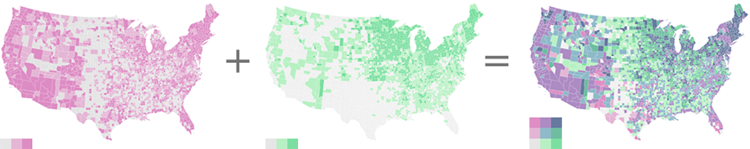
\includegraphics[width=0.7\textwidth]{images/background/js_choroMath.png}
    \caption[Bivariate Choropleth Maps]{Choropleth Maps.\protect\footnotemark[26]}
    \vspace{-10pt}
    \label{fig:choropleth}
\end{figure}
%
As seen, color blending can help conveying information but, at the same time, it can undermine the accuracy of
the perception if too many variables are shown at the same time, or even if there exists scales with too many
interpolations. Some techniques have been under research to provide a curated approach to color perception
tasks, which can be combined with color blending also.
%
\subsection{Color Blending Alternatives}
Besides simple color blending techniques, researchers have been developing techniques in order to convey
even more detailed and accurate information. Examples of these studies are:
a technique of color weaving and a hue-preserver color blending technique, covered in this section.
%
\subsubsection{Color Weaving}
%
\begin{wrapfigure}[10]{r}{0.25\textwidth}
	\centering
    \vspace{-\baselineskip}
    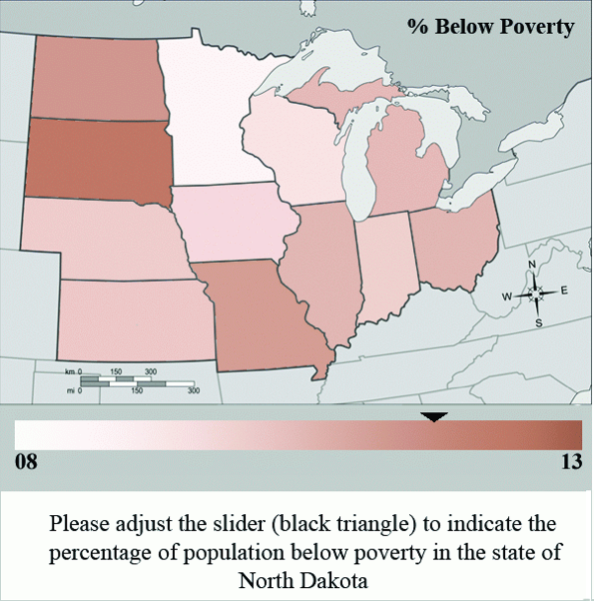
\includegraphics[width=0.25\textwidth]{images/background/WeavingTest1.png}
    \caption[Color Weaving - First Study]{Example of a Map.
    \protect\cite{Hagh-Shenas2007}}
    \label{fig:weaving2}
\end{wrapfigure}
%
One of the challenges of multivariate visualization
is to clearly show different layers of information with color patterns, with no doubt to the user: as
composing different layers on top of each other, most of the time it creates colors and patterns which
do not have direct or significant meaning. Urness \emph{et al.} proposed new insights and introduced new
techniques for using color and texture in a effective way, to convey information about two-dimensional
scalar and vector distributions \cite{Urness2003}: beside other techniques, the authors have introduced the concept
of color weaving, a color blend technique that presents original colors separately, composing a colored
mesh with a fine-grain texture. Comparing to the tradicional color blending, the latter is a simple flat
color used to illustrate the mix of different entities with different values, whereas the new one
combines multiple scalar single-hue-encoded distributions, computed over a common field, to form a
multi-colored line integral convolution tapestry, in which multiple color combinations are represented
explicitly via adjacent lines in a texture, rather than overlaying multiple layers of single color. \par
This technique was vastly studied by Hagh-Shenas \emph{et al.} \cite{Hagh-Shenas2007}. These researchers created a
set of experiments, in which the user was questioned over a state map of U.S.A., reading it and giving answers
that would be statistically analyzed. \par
%
The authors concluded that Color Blending and Color Weaving have a common problem: the background color and the
surrounding color can change the appearance of a color. These studies also led to conclude that the technique
of color weaving is substantially effective for multivariate visualization; combinations of 2, 3 or 4 different
data variable remain error rate low, but with 6 the rate begins to rise. It was not found any significant advantage,
for both color blending and color weaving, in using more separated hues in CIE L*a*b*. Finally, a relevant conclusion of
this study is that hues and luminance play different roles, since the observers estimate the lightness
value of each variable in question and hue is only used for distinguishing the variables from each other.
%
\subsubsection{Hue-Preserving Color Blending}
%
Transparency is almost indispensable when visualizing three dimensional structures, since it is one way to
alleviate the observer’s visual barriers.
In 2009, Chuang et al. tried to combine color and transparency when visualizing volume information,
introducing the idea of preserving the of preserving the hue of the original color when blending \cite{Chuang2009}. \par
Perceptual transparency is the perception of an object being in front of another
background object: the authors created an approach that is not subject to any type of physical constraint, but can be
formulated as an algebraic model. They have reached a set of design criteria that lead
to an equation which expresses the color addition in Hue-Preserving color blending: $C_{new} = C_{1} \oplus C_{2}$ \par
%
\begin{wrapfigure}[10]{r}{0.4\textwidth}
	\centering
    \vspace{-10pt}
    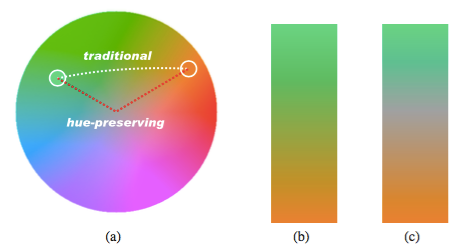
\includegraphics[width=0.4\textwidth]{images/background/HuePreserving.png}
    \caption[Hue-Preserving Color Blending - Orange-Green Scale]{(a) Regular and
    Hue-preserving color blending. (b) Traditional alpha blending between teal and orange. (c) Hue-Preserving
    color blending ofteal and orange.
    \protect\cite{Chuang2009}}
    \label{fig:huepreserving1}
\end{wrapfigure}
%
There were some requirements that Hue-Preserving sum had to meet:
    \begin{itemize}
			\setlength\itemsep{0.01em}
    \item The luminance of $\left(C_{1} \oplus C_{2}\right)$ should be identical to the sum of the
    luminance of C1 and C2.
    \item The hue of $C_{new}$ is either equal to the hue of C1 or C2: $Hue(C_{new}) \in \left\{Hue(C_{1}),
    Hue(C_{2})\right\}$. The hue of $C_{new}$ is chosen as the dominant hue of the two colors $C_{1}$ and $C_{2}$. The
    dominant color is the one whose hue would be closest to the blended color in traditional color summation.
    When the dominant color, and thus the final hue, is to change, $C_{new}$ should go though the gray point
    with vanishing saturation, so that even an abrupt change of hue does not imply a discontinuity in
    chromaticity, as seen on Figure \ref{fig:huepreserving1}.(c).
    \end{itemize} \par
		%
The goal of modifying the sum operator is that, when two colors are mixed, the resultant color only
contains the hue of one of the mixed colors, the dominant one. This technique can be divided into two
pieces, either occurring one or another: \textbf{A:} The blending from one input color $C_{1}$ towards the gray axis,
keeping the hue of $C_{1}$, and \textbf{B:} The blending from the other input color $C_{2}$ towards the gray axis,
keeping the hue of $C_{2}$. \par
The hue from the dominant color does not change: it is the hue from the non-dominant that is modified
(but only the saturation and luminance) until it reaches a complementary color to dominant. By adding
the opponent colors, the mixing moves towards the gray point and it is guaranteed that the original hue
does not change; this also guarantees that this method generates exactly the same result as the
tradicional blending, when mixing opponent colors.
However, there are some disadvantages: gray colors in hue-preserving blended images can be confusing as
gray can come from blending various hues (as on Figure \ref{fig:examples}), and this technique of blending
colors is order-dependent, since
blending colors in different blend orders can produced different results.
%
\begin{figure}[!h]
  \centering%
  \begin{minipage}{0.3\textwidth}
    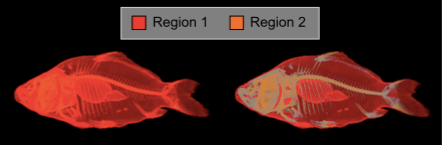
\includegraphics[width=\linewidth]{images/background/HuePreserving_3.png}
  \end{minipage}%
  \hspace{0.2\textwidth}%
  \begin{minipage}{0.3\textwidth}\centering
    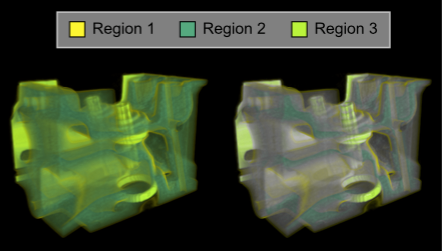
\includegraphics[width=\linewidth]{images/background/HuePreserving_4.png}
  \end{minipage}%
  \caption[Hue-Preserving Color Blending Examples]{Example of a Regular Color Blending (left side of each image) \emph{versus}
    Hue-Preserving Color Blending (right side of each image). \protect\cite{Chuang2009}}
  \label{fig:examples}
\end{figure}
%
\subsubsection{Other Investigation in Color Usage}
%
Colormaps are commonly used in many domains in computer science, \emph{e.g.}, computer graphics, visualization, computer vision and image processing.
Particularly in visualizations, as they are able to improve the efficiency and effectiveness of data perception and therefore allow more insights
into the data. Therefore, it is crucial for visualization designers and users to understand colormap generation techniques as well as the general
rules for choosing appropriate colormaps for specific data. Zhou and Hansen \cite{Zhou2016} provide a way to classify colormapping techniques into
a taxonomy for readers to quickly identify the appropriate techniques they might use, classifying representative visualization techniques that
explicitly discuss the use of colormaps. These authors gathered the investigation performed by other researchers in this paper. There are a set of
standards for a good colormap, namely \ul{order} (colors should have perceptual orders in a colormap), \ul{uniformity and representative distance}
in which perceived color distances should match actual differences between the data they represent; and \ul{boundaries} where colors should not
create false perceived boundaries in data. Additionaly, the authors classify colormap generation as: \textbf{procedural, user-study based, rule
based} and \textbf{data-driven}, which shows that with a deeper understanding of colors and data, as well as the advent of more powerful computation,
methods for colormap generation have evolved from procedurally designing a default colormap for all data, into more intelligent data-driven approaches
as the state-of-the-art. \par
%
\begin{wrapfigure}[18]{r}{0.35\textwidth}
	\centering
    \vspace{-10pt}
    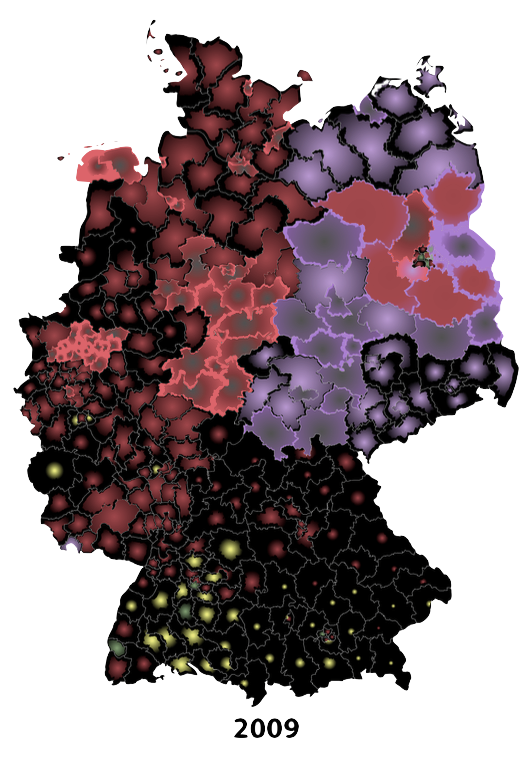
\includegraphics[width=0.35\textwidth]{images/background/stoffel.png}
    \caption[Stoffel's Technique to Visualize Proportions with Hues.]{Stoffel's Technique to Visualize Proportions with Hues. \protect\cite{Stoffel2012}}
    \label{fig:stoffel}
\end{wrapfigure}
%
Stoffel, Janetzko and Mansmann introduced a new technique \cite{Stoffel2012} for visualizing proportions in categorical data; in particular, they combine bipolar colormaps
with an adapted double-rendering of polygons to simultaneously visually represent the first two categories and the spatial location; as the example given
in their paper, this enables the recognition of close election results as well as clear majorities, or other similar subjects. Representing data variables
in a map makes the choice of visual variables more challenging, as the most important variable, namely position, is already occupied representing the geographic location:
therefore, when showing values of a categorical data set, it stands to reason using color hue to represent the different categories (in the particular case of this
example, each party). The difference in this technique resides in reusing the visual variable shape by placing a shrunk polygon of the specific shape
on top of the original polygon, to express the distance to the second ranked category: if the distance between both polygons is very large, then the winner is
far ahead of the second one, and the inner polygon will be very small, and vice versa. While attributing a color to categories, the outer polygon is filled in
the color of the winning party, and a gradient fill is applied from the color of the second party (inner) to the color of the winner (outer). However, there is one
issue addressed here, namely the visibility of the first ranked category in cases of a very tight result: in this case the outer polygon would diminish and could
not be visible at all; also, this techniwue cannot handle different sized polygons very well as the visual salience of large polygons will always exceed the
salience of small polygons. Figure \ref{fig:stoffel} exemplifies a map for Germany's 2009 Elections, showing the results crossed for all parties.
%
\section{Discussion}
\label{sec:background_discussion}
%
The goal of this research is to understand how people perceive the blending of particular colors and if perceived,
in which terms do they understand the blended color. We have conducted an investigation to realize what is related to
the act of perceiving color and how it is judged.  \par
The usage of color blending is hugely related to the fact that color is great to convey information and messages,
but there has not been quite an extensive analysis about how people react to blends of color, having in mind also
cultural patterns which could be tested. Gama and Gonçalves have tested the color blending for Data Visualization \cite{Gama20141},
concluding that users can detect mixtures with higher success rates for colors which represent to smaller angles
in the CIE-L*C*h* color wheel, but users found it hard to perceive the colors that were mixed during the study.
The users also chose the CMYK Color Model as having the smoothest transition of color. It should be take into
consideration that, although the sample is large, there is a considerable gap between genders, which should be
more well balanced in future work. \par
On the other hand, Gama and Gonçalves tested how the users perceive relative amounts of color \cite{Gama20142}, realizing that they happen to perceive most
colors correctly regarding the pair (Red-Yellow) and other extreme colors, and at most 5 colors should be presented
to the user when blending colors, so that the relative amount of each color component is perceivable by the users.
However, in none of the studies were considered cultural differences and standards and the sample of users was
quite reduced to European citizens living in Europe. In further studies, a larger sample should be
considered. \par
Finally, there were studied some alternative techniques to color blending which could be further tested, such
as \textbf{Hue-Preserving Color Blending and Color Weaving}, by Hagh-Shenas \cite{Hagh-Shenas2007}. In this technique, a textured mesh presents the original
colors that were mixed to create a resulting color, using a Noise function to create the pattern in which the
relative amounts of colors were represented. It was also studied by Stoffel and felow researchers \cite{Stoffel2012} a Technique
to present more than one variable at time, in a map, using hues: it attributed a color to each shape of the map and placed a shrunk polygon of the specific shape
on top of the original polygon, to express the distance to the second ranked category. Then, the polygons were colored according to
a pre-defined mapping of colors and categories: the outer polygon is filled with the color of the winning category, and a gradient fill is
applied from the color of the second category (inner) to the color of the winner (outer). \par
%
Considering these conclusions drafted from both the theoretical background and research related work, we can divide the
possible questions which remain unaswered as follows:
%
\begin{itemize}
	\setlength\itemsep{0.1em}
	\item \textbf{Questions raised Before}
    \begin{itemize}
    	\setlength\itemsep{0.01em}
			\item Will perceived colors correspond to a particular fixed angular value, in the color wheel?
      \item Which is the best formula to blend colors, in each color model? Is it linear interpolation or another?
      \item In the case in which 3 colors are blended, do observers realize all colors at the same time or do they
			decompose the mixture, firstly in a mixture of two colors and then a blending of a third color?
      \item What is the best way to present color, without influencing color perception?
      \item Does the user, in fact, understands which colors are involved in a mixing?
		\end{itemize}
  \item \textbf{Perception Questions}
    \begin{itemize}
    	\setlength\itemsep{0.01em}
    	\item Does the order in which colors are mixed, influence mental mixing models? Are there common patterns among mixing orders?
      \item Do shapes and proximity, influence how color is perceived?
      \item Until which extent does background influence the perception of a subject, in particular a blended color?
      \item If color parameters like Saturation, Value or Luminance change in a blending, does it modify color blending perception?
    \end{itemize}
  \item \textbf{Information Visualization Questions}
    \begin{itemize}
    	\setlength\itemsep{0.1em}
			\item Do continuous scales yield better results than discrete color scales?
      \item What is the influence of nominal color scales in perception?
      \item What are the results if no color scale is presented to guide the user?
		\end{itemize}
  \item \textbf{Cultural Questions}
    \begin{itemize}
    	\setlength\itemsep{0.01em}
			\item Does the gender really influences how the color is perceived? Is it possible to observe a significant gap between
			male and female answers?
			\item Is it possible to observe significant differences in observation, depending on user's cultural background?
		\end{itemize}
\end{itemize} \par
%
Although we have rised all these questions which do not have met its answer, only a portion of them will meet their answers,
since this is Master Thesis Research Problem. However, there is a set of these questions which was considered crucial and, consequently,
had more priority above others: it was this set which was the focus of our studies. We performed \textbf{one user study} and,
in the following sections, it is covered the entire description of the solution developed for this color study, the conditions in which
the study is ideally performed and analyze the results collected from it. In the end, we will perform a discussion of results and deduce
some possible implications for the Information Visualization research area.
%
